% The Source Code of Science — a doctoral course note.
% Build with:  latexmk -xelatex main.tex   (or: make)
\documentclass[11pt,oneside]{report}

% Preamble for "The Source Code of Science" — SWH-branded LaTeX course note.
% Engine: xelatex.  Bibliography: biblatex + software-biblatex (biber).

% --- Fonts (xelatex) ------------------------------------------------------
\usepackage{fontspec}
\setmainfont{TeX Gyre Pagella}
\setsansfont{TeX Gyre Heros}
\setmonofont{Latin Modern Mono}[Scale=0.92]
\usepackage{microtype}

% --- Page geometry: wide outer margin for key-takeaway margin notes -------
\usepackage[a4paper,top=2.6cm,bottom=2.6cm,inner=2.4cm,outer=4.2cm,
            marginparwidth=3cm,marginparsep=0.6cm,headheight=15pt,includehead]{geometry}

% --- Colours, graphics, boxes ---------------------------------------------
\usepackage{graphicx}
\usepackage{array}
\usepackage{booktabs}
\usepackage{tabularx}
\usepackage{longtable}
\usepackage{xcolor}
\definecolor{swhaccent}{HTML}{C8102E}
\definecolor{swhdark}{HTML}{2B2B2B}
\definecolor{swhbg}{HTML}{F7E9EC}
\usepackage[most]{tcolorbox}
\usepackage{marginnote}
\usepackage{enumitem}
\usepackage{etoolbox}

% --- Classier headings (titlesec) -----------------------------------------
\usepackage{titlesec}
% Chapter opener: large accent numeral, dark title, a hairline accent rule under.
\titleformat{\chapter}[display]
  {\normalfont\sffamily}
  {\fontsize{52}{52}\selectfont\bfseries\color{swhaccent}\thechapter}
  {6pt}
  {\Huge\bfseries\color{swhdark}}
  [\vspace{4pt}{\color{swhaccent!85}\titlerule[1.1pt]}]
% Numbered chapters start a touch higher (also reclaims wasted top space).
\titlespacing*{\chapter}{0pt}{6pt}{22pt}
% Unnumbered chapters (About / Colophon): title + the same accent rule, no numeral.
\titleformat{name=\chapter,numberless}[display]
  {\normalfont\sffamily}{}{0pt}
  {\Huge\bfseries\color{swhdark}}
  [\vspace{4pt}{\color{swhaccent!85}\titlerule[1.1pt]}]
\titleformat{\section}
  {\normalfont\sffamily\Large\bfseries\color{swhdark}}
  {\color{swhaccent}\thesection}{0.7em}{}
\titleformat{\subsection}
  {\normalfont\sffamily\large\bfseries\color{swhdark}}
  {\color{swhaccent}\thesubsection}{0.6em}{}

% --- Running heads + provenance footer (fancyhdr) -------------------------
\usepackage{fancyhdr}
% Build-time git state (written by .latexmkrc); fallback if built by hand.
\InputIfFileExists{gitinfo.tex}{}{}
\providecommand{\gitinfo}{unknown}
% One reusable provenance line: author, title, licence, build date, git state.
\newcommand{\provenancefoot}{\footnotesize\sffamily\color{swhdark!60}%
  Roberto Di Cosmo\,\textperiodcentered\,\textit{The Source Code of Science}%
  \,\textperiodcentered\,CC\nobreakdash-BY\nobreakdash-4.0%
  \,\textperiodcentered\,\today\,\textperiodcentered\,\texttt{g:\gitinfo}}
\newcommand{\chapmarkfmt}[1]{\thechapter\;\textperiodcentered\;#1}
\renewcommand{\chaptermark}[1]{\markboth{\chapmarkfmt{#1}}{}}
\pagestyle{fancy}
\fancyhf{}
\renewcommand{\headrulewidth}{0.4pt}
\renewcommand{\footrulewidth}{0pt}
\fancyhead[L]{\small\sffamily\itshape\color{swhdark!75}\nouppercase{\leftmark}}
\fancyhead[R]{\small\sffamily\color{swhdark!75}\thepage}
\fancyfoot[C]{\provenancefoot}
% Chapter-opening pages use 'plain': no header, but keep the footer + page number.
\fancypagestyle{plain}{%
  \fancyhf{}\renewcommand{\headrulewidth}{0pt}%
  \fancyfoot[C]{\provenancefoot}\fancyfoot[R]{\small\sffamily\color{swhdark!75}\thepage}}

% --- Page fill: pack floats, honest ragged bottoms (fewer short pages) -----
\renewcommand{\topfraction}{0.9}
\renewcommand{\bottomfraction}{0.8}
\renewcommand{\textfraction}{0.08}
\renewcommand{\floatpagefraction}{0.75}
\setcounter{topnumber}{3}
\setcounter{bottomnumber}{2}
\setcounter{totalnumber}{5}
\raggedbottom
% Discourage widows/orphans; soak up the few tight lines instead of overflowing.
\widowpenalty=10000
\clubpenalty=10000
\setlength{\emergencystretch}{2em}

% --- Links (load before biblatex) -----------------------------------------
\usepackage{hyperref}
\hypersetup{colorlinks=true,linkcolor=swhdark,citecolor=swhaccent,
            urlcolor=swhaccent,breaklinks=true}

% --- Bibliography: the software-aware style -------------------------------
\usepackage{csquotes}
\usepackage[backend=biber,style=numeric,sorting=nyt,datamodel=software]{biblatex}
\usepackage{software-biblatex}
\ExecuteBibliographyOptions{halid=true,swhid=true,swlabels=true,vcs=true,license=true,crossrefexpansion=conditional}
\addbibresource{references.bib}

% --- Pedagogical devices --------------------------------------------------
% Hands-on lab box.
\newtcolorbox{handson}[1][Hands-on]{%
  breakable, enhanced, colback=swhbg, colframe=swhaccent, coltitle=white,
  fonttitle=\bfseries\sffamily, title={\,#1}, sharp corners=downhill,
  boxrule=0.6pt, left=2.2mm, right=2.2mm, top=1.4mm, bottom=1.4mm}

% Learning-objectives box (chapter openers).
\newtcolorbox{objectives}{%
  breakable, enhanced, colback=swhbg!45, colframe=swhdark,
  fonttitle=\bfseries\sffamily, title={Learning objectives}, sharp corners=downhill,
  boxrule=0.4pt, left=2.2mm, right=2.2mm, top=1mm, bottom=1mm}

% Generic titled callout (boilerplate, executive summary, governance, do-one-thing).
\newtcolorbox{callout}[1]{%
  breakable, enhanced, colback=swhbg!25, colframe=swhdark,
  fonttitle=\bfseries\sffamily, title={#1}, sharp corners=downhill,
  boxrule=0.4pt, left=2.2mm, right=2.2mm, top=1mm, bottom=1mm}

% Per-lab metadata line (time / prereqs / mode), set under a Hands-on title.
\newcommand{\labmeta}[1]{{\footnotesize\sffamily\itshape\color{swhdark!75}#1}\par\smallskip}

% Key-takeaway margin note.
\newcommand{\takeaway}[1]{\marginnote{\footnotesize\sffamily\itshape\color{swhaccent}#1}}

% Reading-path marks for the audience guide (core / skim / skip).
\newcommand{\pathcore}{\tikz[baseline=-0.5ex]\fill[swhaccent](0,0)circle(1.8pt);}
\newcommand{\pathskim}{\tikz[baseline=-0.5ex]{\draw[swhaccent,line width=0.4pt](0,0)circle(1.8pt);%
  \fill[swhaccent](0,0)--(90:1.8pt) arc(90:270:1.8pt)--cycle;}}
\newcommand{\pathskip}{\textcolor{swhdark!30}{\textperiodcentered}}

% SWHID display helper (small monospace, allows breaks).
\newcommand{\swhid}[1]{\texttt{\small #1}}

% Readable-core, full-qualified-link: show a short/core SWHID as the visible text,
% but carry the full qualified SWHID --- resolver prefix and all --- in the hyperlink.
% Usage: \swhref{visible (core) swhid}{full qualified swhid, without the resolver prefix}
\newcommand{\swhresolver}{https://archive.softwareheritage.org/}
\newcommand{\swhref}[2]{\href{\swhresolver#2}{\swhid{#1}}}
% Same, but with a long, line-breakable visible text (\nolinkurl breaks at ; = : /).
\newcommand{\swhreflong}[2]{\href{\swhresolver#2}{\small\nolinkurl{#1}}}

% Diagrams.
\usepackage{tikz}
\usetikzlibrary{positioning,arrows.meta,shapes.geometric,fit,backgrounds,calc}

% Self-archival stamp (see the Colophon and the Makefile `swhid` target).
% A document cannot contain its own SWHID; `make swhid` injects it, at build
% time, into a throwaway swhid.tex consumed only by the stamped (non-committed)
% PDF. A plain `make` leaves \thisswhid empty -> the Colophon shows a placeholder.
\providecommand{\thisswhid}{}
\ifdef{\STAMPSWHID}{\InputIfFileExists{swhid.tex}{}{}}{}

% --- Title-page command ---------------------------------------------------
\newcommand{\swhtitlepage}{%
  \begin{titlepage}
  \centering
  
\includegraphics[height=2.0cm]{logos/SWH-logo.pdf}\par\vspace{2.2cm}
  {\Huge\bfseries The Source Code of Science\par}\vspace{0.6cm}
  {\Large Archiving, Referencing and Reproducing Research Software\par}\vspace{0.3cm}
  {\large\itshape a doctoral course --- beyond FAIR data\par}\vspace{2.4cm}
  {\large Roberto Di Cosmo\par}\vspace{0.2cm}
  {\large Software Heritage\par}\vfill
  {\small This work is licensed under a Creative Commons
   Attribution~4.0 International License (CC-BY-4.0).\par}
  {\small \today\par}
  \end{titlepage}}


\begin{document}

\swhtitlepage

% --- Abstract / how to read this note ------------------------------------
\chapter*{About this note}
\addcontentsline{toc}{chapter}{About this note}
This note is a doctoral-level course on managing the \emph{source code} of research:
how to archive it for the long term, reference it at the right granularity, describe and
cite it, and use it to make computational results reproducible. It is built on Software
Heritage\footnote{In the interest of transparency: the author helped found Software Heritage,
co-developed the \texttt{biblatex-software} style used here, and contributed to the \textsc{swhid}
standard; the recurring worked example (the Parmap library) is also his. The argument is meant to
stand on its evidence, and the sources cited throughout are independent.} and the \textsc{swhid} ---
an identifier computed from the code itself, defined in Chapter~\ref{ch:identifiers} and now the
international standard ISO/IEC~18670:2025. It addresses
the FAIR principles and then goes \emph{beyond} them, following the CODE-beyond-FAIR roadmap for
research software~\autocite{NatureSD2026}. The acronyms in this paragraph are all explained, in
order, in the chapters that follow; nothing here needs to be known in advance.

The note is meant to be read \emph{and} done: each practical chapter ends with a
\textbf{Hands-on} box. Margin notes flag the key takeaways.

\begin{callout}{In one page (for the busy reader)}
\small
\textbf{The claim.} Source code is a first-class research output, but the habit of depositing a
\texttt{.zip} with a DOI fails it: a DOI certifies a landing page, not the bytes; the deposit can
change, has no granularity, and discards history. The fix is to archive the living repository in
\textbf{Software Heritage} and reference it with a \textbf{\textsc{swhid}} --- an identifier computed
from the content itself, recomputable and verifiable offline, and the international standard
ISO/IEC~18670.

\textbf{The evidence.} The archive holds the development history of more than 28~billion source
files from over 430~million projects. The \textsc{swhid} is already accepted by ACM for the
\emph{Artifacts Available} badge; \emph{eLife} has auto-archived every article's code since 2020;
HAL, IPOL, swMATH, and Episciences are wired in; UNESCO, EOSC, France's National Plan, and the ANR
all point research software at Software Heritage.

\textbf{What to do.}
\emph{Researchers}: archive your code, cite it with a \textsc{swhid} (Chapter~\ref{ch:ardc}).
\emph{Editors / AEC chairs}: require a \textsc{swhid} for the \emph{Available} badge --- a reviewer
can verify it offline (Chapter~\ref{ch:repro}, with a ready call-for-artifacts box).
\emph{Funders / policy makers}: name Software Heritage and the \textsc{swhid} in conditions and
policy (Chapter~\ref{ch:outlook}, with a model clause and a governance/sustainability note).
\end{callout}

\newcommand{\pathcore}{\tikz[baseline=-0.5ex]\fill[swhaccent](0,0)circle(1.8pt);}
\newcommand{\pathskim}{\tikz[baseline=-0.5ex]{\draw[swhaccent,line width=0.4pt](0,0)circle(1.8pt);%
  \fill[swhaccent](0,0)--(90:1.8pt) arc(90:270:1.8pt)--cycle;}}
\newcommand{\pathskip}{\textcolor{swhdark!30}{\textperiodcentered}}

\clearpage
\begin{samepage}
\begin{callout}{How to read this note, by audience}
\small Not everyone needs every chapter. Pick a row and follow it; the rest can wait. The chapters
do build on one another --- the \textsc{swhid} (4) rests on the data model (3), and the practical
core (5) uses both --- so a skipped chapter is there when you need it.
\smallskip

\centering
\renewcommand{\arraystretch}{1.25}
\begin{tabular}{@{}l*{7}{c}c@{}}
\toprule
\textbf{Reader} & \textbf{1} & \textbf{2} & \textbf{3} & \textbf{4} & \textbf{5} & \textbf{6} & \textbf{7} & \textbf{App.}\\
\midrule
Researcher \emph{(just do it)} & \pathcore & \pathskip & \pathskip & \pathskim & \pathcore & \pathskip & \pathskip & A\\
Reviewer / editor / AEC        & \pathcore & \pathskip & \pathskip & \pathcore & \pathskim & \pathcore & \pathskip & ---\\
Funder / policy maker          & \pathcore & \pathskip & \pathskip & \pathskip & \pathskip & \pathskip & \pathcore & E\\
Full course / student          & \pathcore & \pathcore & \pathcore & \pathcore & \pathcore & \pathcore & \pathcore & all\\
\bottomrule
\end{tabular}

\smallskip
{\footnotesize \pathcore~core \quad \pathskim~skim / optional \quad \pathskip~skip. \quad
\textbf{1}~Why \enspace \textbf{2}~Beyond FAIR \enspace \textbf{3}~Foundations \enspace
\textbf{4}~The \textsc{swhid} \enspace \textbf{5}~\textsc{ardc} \enspace
\textbf{6}~Reproducibility \enspace \textbf{7}~Policy.}
\end{callout}
\end{samepage}

\tableofcontents

% --- Chapters ------------------------------------------------------------
\chapter{Why these notes}
\label{ch:why}

\begin{objectives}\small
\begin{itemize}[nosep,leftmargin=*]
  \item place software as a first-class research output, beside publications and data;
  \item name the two things at stake --- reproducibility and preservation;
  \item see why a software forge is not an archive.
\end{itemize}
\end{objectives}

Software source code is a precious, unique form of knowledge. It can be turned, almost
instantly, into something a machine will execute; and yet it is written to be read by people.
As Harold Abelson put it in 1985, \enquote{programs must be written for people to read, and
only incidentally for machines to execute}. A program is a human creation in the same sense as
an article or a proof --- a record of how its authors understood a problem and chose to solve
it --- and in research it is, more and more, the place where the actual science happens: the
model that was simulated, the data that were cleaned, the figure that was produced.

\takeaway{Publications, data, \emph{and} software: source code is a first-class research output.}

And yet, when a published result rests on code, that code is too often the first thing we lose.
The article is archived, typeset, given a DOI; the data, increasingly, are deposited in a
repository; the software --- the one artifact that actually produced the numbers --- is left on
a personal web page, in a forge that may close next year, or nowhere at all. These notes are about
taking that software as seriously as we take the paper, and about the concrete,
already-available practice that lets you do so --- starting with your next paper.

\section{Software as the third pillar of open science}

Open science rests on three pillars: publications, data, and software. The first two have had
their revolutions. Open access freed the article; the FAIR principles and a dense network of
repositories gave research data a home, identifiers, and metadata. Software, meanwhile, was
treated as a mere means to an end --- a tool you used and then forgot --- rather than as a
research output in its own right.

This is no longer tenable, and the numbers say so. Across \emph{every} discipline, from
mathematics to biology, from physics to the social sciences, a growing share of published work
now depends on software the authors wrote themselves~\autocite{osec_2022} (Figure~\ref{fig:os-monitor}).
When the code \emph{is} the experiment, pretending it is a detail does not make it one.

\begin{figure}[htbp]
  \centering
  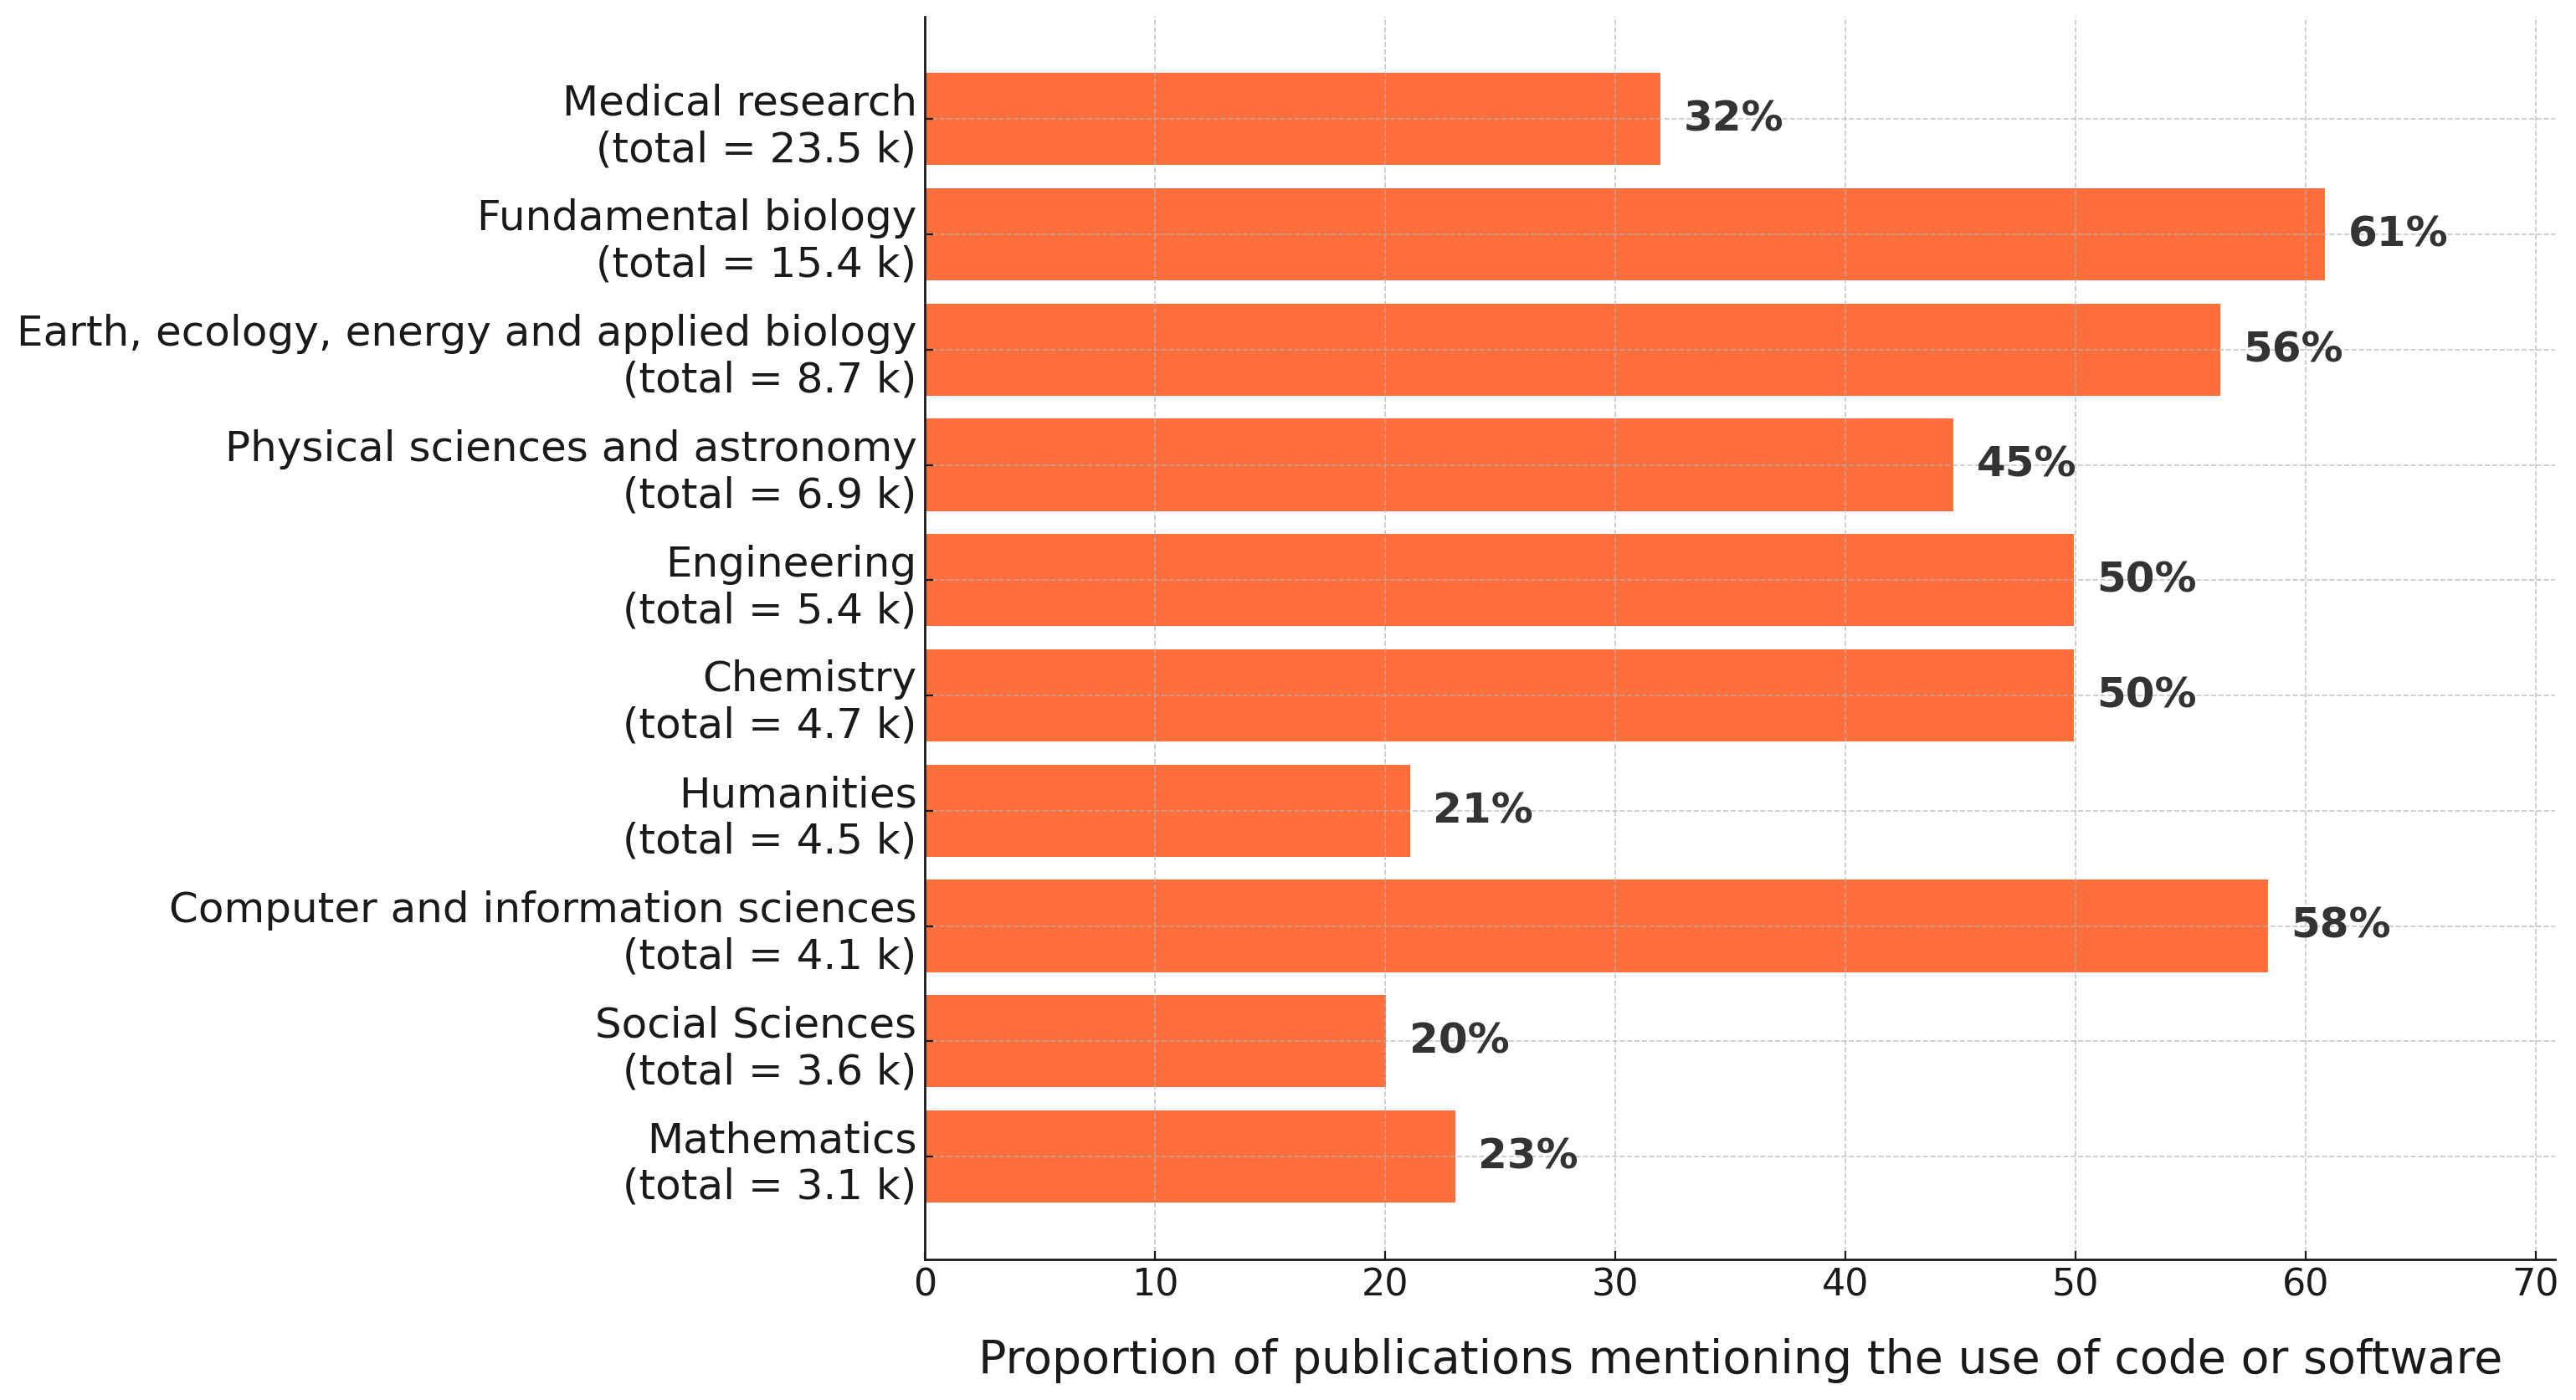
\includegraphics[width=\linewidth]{figures/french_os_monitor-use-2025.png}
  \caption[Software across all disciplines]{Across every discipline, a substantial and growing
  share of research articles produces or uses software. \emph{Source:} French Open Science
  Monitor, 2025 edition.}
  \label{fig:os-monitor}
\end{figure}

What makes software special is also what makes it easy to mishandle: it is at once executable
and human-readable; it \emph{evolves}, often over decades, so that its development history is
part of its meaning; and it never stands alone, resting instead on a deep web of other software
it depends on (Figure~\ref{fig:matplotlib-deps}). These are not the properties of a dataset ---
and, as we will see in the next
chapter, they are exactly the properties that the familiar, data-shaped recipes fail to
respect. Software is not data; it is a first-class citizen of the scientific record, and it
deserves to be treated as one.

\begin{figure}[htbp]
  \centering
  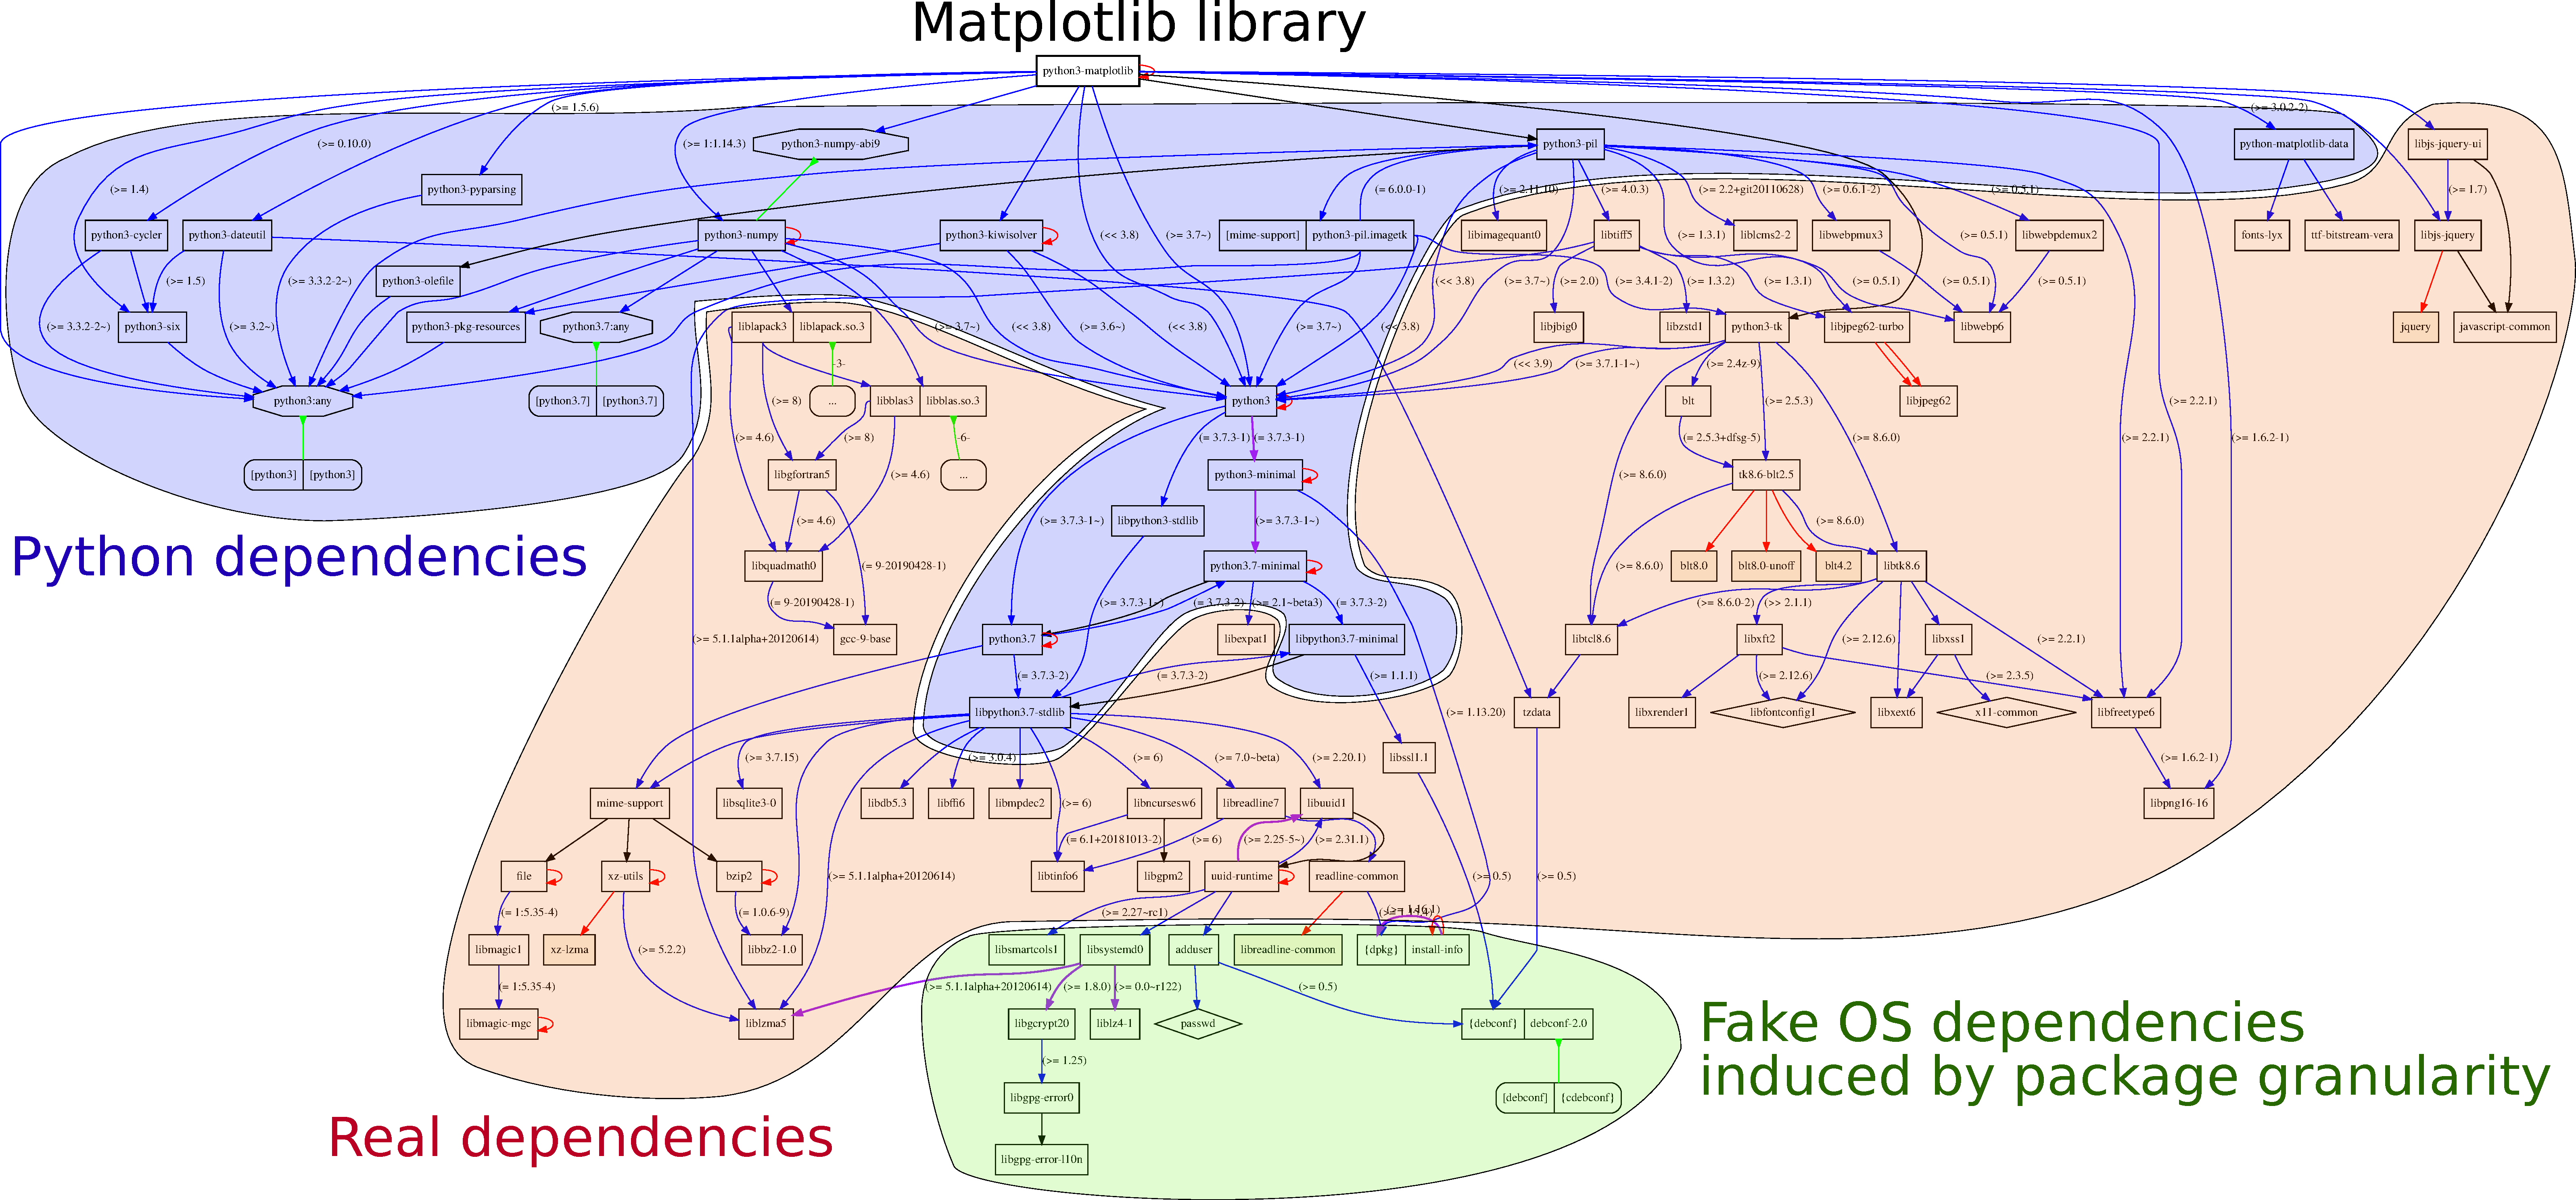
\includegraphics[width=\linewidth]{figures/python3-matplotlib.pdf}
  \caption[The dependency web of a single library]{No software stands alone. The dependency
  graph of the \texttt{matplotlib} plotting library: blue marks its Python-level dependencies,
  orange the real system libraries beneath, green the artefacts of packaging
  granularity~\autocite{SWHecosystems2023}. The individual labels are not meant to be read; the
  point is the \emph{density} --- a single research tool already rests on a deep web of other
  software, none of which the data-deposit model knows how to keep.}
  \label{fig:matplotlib-deps}
\end{figure}

\section{What is at stake}

The two most visible stakes are worth naming plainly, first.

The first is \emph{reproducibility}. A computational result is only as solid as our ability to
get hold of the exact code that produced it and run it again --- not code \emph{like} it, not a
later version with the bug quietly fixed, but \emph{that} code, at \emph{that} revision. We will
return to the dispiriting state of the art in Chapter~\ref{ch:repro}; for now it is enough to
say that, far too often, the code behind a published figure cannot be found, cannot be built, or
cannot be told apart from a dozen neighbouring versions.

The second is \emph{preservation}, and here a single slogan does most of the work: \emph{forges
are not archives}. GitHub, GitLab, and their kin are wonderful places to \emph{develop}
software; they make no promise whatsoever to \emph{keep} it. That promise has been tested, and
broken, more than once: Google Code and Gitorious shut down in 2015, putting roughly a million
repositories at risk; Bitbucket deleted more than 250,000 Mercurial repositories in 2020. The
half-life of a URL cited in the scholarly literature is about four years. Every one of those
losses is a hole in the web of knowledge --- a paper that points at code which is no longer
there.

\takeaway{Forges are for developing code; they make no promise to keep it.}

But reproducibility and preservation are only the most visible of a \emph{plurality} of needs ---
and those needs stack, scale by scale, each resting on the one beneath it.

A \emph{researcher} needs to archive and reference the exact code behind each result, so it can be
retrieved and re-run; to find and reuse the software of others; and --- not least --- to get
\emph{credit} for the software they build themselves, as for any other research output.

A \emph{laboratory or team director} needs to know what the group actually produces: to track its
software contributions, fold them into activity reports and a public software page, and not lose
them when the student who wrote them moves on.

A \emph{research organization} --- a university president, a funding agency --- needs to know its
\emph{software assets} at all: for technology transfer, for honest impact metrics, for funding
strategy, and for the fair career evaluation of the people who write software.

And here is the point that organises this whole note. Every one of these needs, from the lone result
to the institutional dashboard, rests on the same minimal foundation --- four things you must be
able to do to a piece of software: \textbf{archive} it (so it can be retrieved), \textbf{reference}
it exactly (so it can be identified), \textbf{describe} it (so it can be discovered and reused), and
\textbf{cite} it (so its authors are credited). Those four verbs --- \textbf{A}rchive,
\textbf{R}eference, \textbf{D}escribe, \textbf{C}ite \& credit, or \textsc{ardc} --- are the floor
beneath all the layers. Get them right, and reproducibility, visibility, and assessment all become
\emph{possible}; skip them, and none of the higher needs can be met, however much metadata or policy
is piled on top.

\takeaway{From the lone result to the institutional dashboard, every need rests on one floor:
\textsc{ardc}.}

And yet, collectively, we have not been taking good care of this precious form of
knowledge~\autocite{SwhCACM2018}. Closing that gap is the whole purpose of these notes.

\section{How to read these notes}

The good news is that \textsc{ardc} is not aspirational: the practice exists, the tools are built,
and you can adopt them today. It rests on two foundations --- the Software Heritage archive, which
preserves the world's source code with its full development history, and the \textsc{swhid}, an
identifier computed \emph{from the code itself} (and now the international standard ISO/IEC~18670)
that lets you point at exactly the code you mean. Chapter~\ref{ch:ardc} makes each of the four verbs
hands-on. We will meet the FAIR principles along the way and then, deliberately, go \emph{beyond}
them, for the reasons the next chapter makes precise~\autocite{NatureSD2026}.

These notes are meant to be read \emph{and} done. The practical chapters end with \textbf{Hands-on}
boxes you run on a repository of your choice --- your own code, a library you depend on, a result
you want to cite. Margin notes flag the one idea worth carrying away from each section; each chapter
opens with its \textbf{learning objectives}; and any unfamiliar term --- \textsc{swhid}, snapshot,
forge, qualified identifier --- is defined in the Glossary (Appendix~\ref{app:glossary}). And these
notes practise what they preach: they are themselves archived in Software Heritage, and the Colophon
shows you how to recompute and verify their own identifier --- the entire workflow, applied to the
very document in your hands.

You do not need to be a computer scientist to use any of this. Different readers will want
different routes through it:

\begin{callout}{Reading paths}
\small Pick a row and follow it; the rest can wait. The chapters do build on one another --- the
\textsc{swhid} (4) rests on the data model (3), and the practical core (5) uses both --- so a skipped
chapter is there when you need it.
\smallskip

\centering
\renewcommand{\arraystretch}{1.25}
\begin{tabular}{@{}l*{7}{c}c@{}}
\toprule
\textbf{Reader} & \textbf{1} & \textbf{2} & \textbf{3} & \textbf{4} & \textbf{5} & \textbf{6} & \textbf{7} & \textbf{App.}\\
\midrule
Researcher                     & \pathcore & \pathskip & \pathskip & \pathskim & \pathcore & \pathskim & \pathskip & A\\
Developer / intern             & \pathskim & \pathskip & \pathskip & \pathskim & \pathcore & \pathskip & \pathskip & A\\
Reviewer / editor / AEC        & \pathcore & \pathskip & \pathskip & \pathcore & \pathskim & \pathcore & \pathskip & ---\\
Funder / policy maker          & \pathcore & \pathskip & \pathskip & \pathskip & \pathskip & \pathskip & \pathcore & E\\
Full course / student          & \pathcore & \pathcore & \pathcore & \pathcore & \pathcore & \pathcore & \pathcore & all\\
\bottomrule
\end{tabular}

\smallskip
{\footnotesize \pathcore~core \quad \pathskim~skim / optional \quad \pathskip~skip. \quad
\textbf{1}~Why \enspace \textbf{2}~Beyond FAIR \enspace \textbf{3}~Foundations \enspace
\textbf{4}~The \textsc{swhid} \enspace \textbf{5}~\textsc{ardc} \enspace
\textbf{6}~Reproducibility \enspace \textbf{7}~Policy.}
\end{callout}

If you write or run code for your research --- whether a few lines of analysis or a library
maintained for decades --- these notes are for you. The tools are ready; the habit is the only thing
missing. Let us build it, starting with your next paper.

\chapter{Software is not data --- and why ``beyond FAIR''}
\label{ch:beyond-fair}

Research software differs from data in kind: it is executable \emph{and} human-readable, it
evolves over time, and it sits atop a deep web of dependencies. The FAIR principles were
designed for data; this chapter shows where they fit research software and where they break,
and introduces the CODE-beyond-FAIR roadmap~\autocite{NatureSD2026}.

\takeaway{FAIR is a starting point, not the destination, for living software.}

\section{The living nature of software}
% TODO draft from: swh-ardc.org::#swnotdata; source-code-different-short.org.
% Figure: a real dependency graph (matplotlib) to make "deep web of dependencies" concrete.
% Assets: common/images/dependency-xkcd-2347.png (CC-BY-NC, attribute) or supply-chain-deps.png;
% better, generate a matplotlib dep graph for a CC-BY-clean figure.

\section{FAIR for software: fit and friction}
% TODO draft: the SNS "What about FAIR?" argument. Refs: barker2022fair4rs (FAIR4RS), 2020GtCitation.
% KEY POINT: the I (interoperable) and R (reusable) of FAIR already have precise, established
% meanings in software engineering --- and they differ from FAIR's data-centric intent. An
% experienced developer hears "interoperable/reusable" and thinks APIs, ABIs, modularity,
% portability --- not metadata. So the FAIR vocabulary actively CONFUSES practitioners. Keep
% what FAIR gets right (Findable + Accessible, delivered by archiving + intrinsic identifiers);
% be explicit that software interoperability/reusability is a distinct, harder, long-studied
% problem, not a metadata checkbox.
\takeaway{For software, \emph{interoperable} and \emph{reusable} already mean something precise
--- and it is not what FAIR means by them.}

\section{The CODE-beyond-FAIR roadmap}
% TODO: tiered roadmap for reusable research software. Ref: NatureSD2026.

\chapter{Foundations: forges, the archive, and the data model}
\label{ch:foundations}

Before we can name a piece of code, we need somewhere that reliably keeps it. This chapter
builds that ground: why software forges are not archives, what a universal archive of source
code collects and how, and the content-addressed data model --- the Merkle DAG --- that makes
the identifiers of the next chapter possible.

\takeaway{A forge is where code is developed; an archive is where it is kept.}

\section{Forges are not archives}
% TODO draft from: forges-not-archives.org::#categories,#oldapproaches,#evidence.
% Link-rot evidence: Google Code/Gitorious (2015), Bitbucket (2020), URL half-life ~4y.

\section{The universal archive}
% TODO draft from: swh-as-infrastructure.org::#oneslide; under-the-hood-pictures.org::#automation.
% What Software Heritage collects and how (listers + loaders), at what scale; non-profit,
% built for the long term. Refs: SwhCACM2018.

\section{The Merkle DAG data model}
% TODO draft from: under-the-hood-pictures.org::#automation; vcs-history.org::#dvcs-to-merkle.
% Content-addressed, deduplicated, history-preserving --- this is what makes intrinsic
% identification possible, and sets up Chapter~\ref{ch:identifiers}.
% Refs: pietri2019graph, SWHecosystems2023.
Software Heritage archives source code with its full development history in a uniform Merkle
DAG~\autocite{ICMS2020,SWHecosystems2023} --- the property that the next chapter turns into an
identifier you can trust.

\chapter{Identifiers for digital objects}
\label{ch:identifiers}

The previous chapter left us with a quietly remarkable fact: in the Software Heritage data model,
every artifact already \emph{has} a name, computed from its own content. Before we put that name
to work, we should be clear about what a name is \emph{for} --- because almost everything people
believe about digital identifiers is tangled in a confusion that a few minutes of care can
dissolve.

\takeaway{Identification is one thing; location, metadata, organization, and curation are four
others. Keep them apart.}

\section{Five concerns hiding behind one word}

When we say that a digital object \enquote{has a DOI}, we are quietly running five different
concerns together. Pulling them apart is the single most clarifying move in this whole subject:

\begin{description}[leftmargin=!,labelwidth=2.5cm,font=\bfseries\sffamily]
  \item[Identification] giving the object a unique name --- the identifier proper.
  \item[Location] a way to \emph{access} or resolve the object. The ISBN names a book; the library
        catalogue tells you which shelf it sits on. Two different jobs.
  \item[Metadata] what is \emph{known about} the object --- authors, title, date --- usually held
        in a registry.
  \item[Organization] who keeps the system coherent: the governance, the registry operator, the
        institutions that keep the lights on.
  \item[Curation] the \emph{quality} of the metadata --- how it is checked and maintained, and who
        decides which objects deserve metadata, or even a name, at all.
\end{description}

Only the first is \emph{identification}. The other four are real and important --- but they are
not the same thing, and most arguments about identifiers turn out to be arguments about one of the
latter four, wearing identification's clothes. One example makes this unforgettable.

\section{``Crossref DOIs are better than DataCite DOIs''}

You will hear this said, and it is worth taking seriously, because it is at once obviously true
and strictly nonsensical --- depending on which of our five concerns you have in mind.

Strictly, it is nonsense. A DOI is a DOI. Crossref and DataCite are both \emph{registration
agencies} accredited by the same International DOI Foundation; both mint identifiers resolved by
the same underlying Handle System~\autocite{Arms01,RFC3650}, through the same \texttt{doi.org}.
They are so much one system that when \texttt{doi.org} suffered an outage in 2015, it took down
\emph{every} agency's DOIs at once. Hand someone a bare DOI and, as a rule, they cannot even tell
you which agency registered it. At the level of \emph{identification}, then, \enquote{better} has
no meaning: the identifiers are the same kind of object, named and resolved in exactly the same
way~\autocite{doifoundation_ra}.

And yet the sentence is not foolish; the people who say it mean something real. They are talking
about \emph{organization} and \emph{curation}. Crossref grew up around the scholarly literature,
DataCite around research data and software; the two run different metadata schemas, serve
different communities, and accumulate metadata of differing richness and quality. But that
richness, as the two organizations themselves put it, \enquote{hinges on what depositing members
actively provide, rather than being automatically generated by the DOI assignment process
itself}~\autocite{crossrefdatacite_metadata}. The quality lives in the organization and its
curation, not in the identifier. So the famous sentence is true and false at the same time: false
about identification, true about everything else --- and it sounds paradoxical only because all
five concerns were crammed into one word. Pull them apart, and the paradox evaporates.

\section{Intrinsic versus extrinsic identifiers}

There is a deeper lesson hiding in that example, and Norman Paskin --- long the voice of the DOI
itself --- put his finger on it: \enquote{Digital Object Identifier} is best read as \emph{digital
identifier of an object}, not \emph{identifier of a digital object}~\autocite{paskin2010digital}.
That distinction is the whole game.

An \emph{extrinsic} identifier --- a DOI, a Handle, an ARK --- is a digital identifier \emph{of}
something, assigned by an organization and recorded in a register. It says nothing about the bytes
it names; it is a pointer whose meaning is maintained, on goodwill, by several parties at once. The
resolution can be repointed; the content at the far end can change; and there is \emph{no intrinsic
way to notice}~\autocite{swhipres2018}. Anyone who has clicked a DOI and met \enquote{not found}
has felt the consequence. Such an identifier delegates to an organization not only \emph{location}
but \emph{identification} itself: without the register, it means nothing.

An \emph{intrinsic} identifier --- a Git commit hash, a \textsc{swhid} --- is an identifier
\emph{of} a digital object, computed from the object's own bytes. It needs no organization to
\emph{mean} something; it needs one only, and separately, to help you \emph{locate} what it names.
As we saw in Chapter~\ref{ch:foundations}, this is exactly what the Merkle construction buys:
identifiers that are gratis, that guarantee \emph{integrity}, and that need \emph{no
middle-man}~\autocite{cise-2020-doi}. Map this back onto our five concerns and the elegance is
plain: an extrinsic identifier entangles identification with location, metadata, organization, and
curation all at once; an intrinsic identifier \emph{separates} identification from all four. That
separation is no technicality. It is the difference between a name you must trust someone to keep,
and a name anyone can check.

\takeaway{An intrinsic identifier is computed from the content; an extrinsic one is assigned by a
registry.}

\section{The SWHID}

The intrinsic identifier for source code is the \textsc{swhid} --- the \emph{Software Hash
Identifier} --- and it is simply the name of a node in the Merkle DAG of the previous chapter. In
its core form it reads \swhid{swh:1:\textit{type}:\textit{hash}}, where the type is one of
\texttt{cnt} (a file's content), \texttt{dir} (a directory), \texttt{rev} (a revision, i.e.\ a
commit), \texttt{rel} (a release), or \texttt{snp} (a snapshot of a whole repository). Thus
\swhid{swh:1:cnt:94a9ed02\ldots} \emph{is} the text of the GPL\,v3 licence, wherever it appears,
and \swhid{swh:1:rel:22ece559\ldots} is release 2.3.0 of the Darktable project --- not a record
pointing \emph{at} them, but a name computed \emph{from} them, that you can recompute yourself.

Identification, though, is not location, and the \textsc{swhid} keeps the two cleanly apart. When
you do want to point a reader into the archive --- to say not merely \emph{which} code but
\emph{where it came from, and in what context} --- you add qualifiers: \texttt{origin} (the URL the
code was harvested from), \texttt{visit}, \texttt{anchor}, \texttt{path}, and \texttt{lines}. The
core name still identifies; the qualifiers merely locate. Appendix~\ref{app:swhid-syntax} gives the
full grammar.

None of this is a private convention. The \textsc{swhid} is an international standard, ISO/IEC
18670:2025, recognised by SPDX, registered with IANA as the \texttt{swh:} URI scheme, and recorded
as Wikidata property P6138~\autocite{isoiec18670}. And it is not theoretical for this very note: as
the Colophon explains, this document is named and verified by its own \textsc{swhid} --- which is
also exactly why it cannot contain that identifier inside itself.

\begin{handson}[Hands-on: watch the name follow the bytes]
\begin{enumerate}[nosep,leftmargin=*]
  \item Compute a content \textsc{swhid} for any file: \texttt{swh identify file.c}.
  \item Change a single byte and recompute --- the identifier changes completely.
  \item Restore the byte; the original identifier returns, to the character. No registry was ever
        consulted, and no authority was asked --- the name simply follows the bytes.
\end{enumerate}
\end{handson}

We now have what the rest of this note needs: a name we can trust, that identifies code exactly,
that anyone can verify without asking permission, and that --- when we choose --- can also tell us
where the code lived. The remaining chapters are about putting that name to work: archiving the
code, referencing it at the right granularity, describing it, and citing it. That practice is
\textsc{ardc}, and it is next.

\chapter{ARDC in practice}
\label{ch:ardc}

We now have everything we need to do the work: an archive that keeps source code for the long
term, and an intrinsic identifier that names exactly the code we mean. This chapter is the
operational heart of the note. It turns the principle ``treat software as a first-class output''
into four concrete verbs you can apply to a repository of your choice --- your own code, a library
you depend on, a result you want to cite. The verbs are \textbf{A}rchive, \textbf{R}eference,
\textbf{D}escribe, and \textbf{C}ite~\&~credit; together they spell \textsc{ardc}, and each ends
with a hands-on lab.

\takeaway{Archive once; then reference at the granularity your claim needs.}

\section{Archive}

Recall the one hard requirement from the CODE roadmap: \emph{publish and archive}. Publishing on a
forge you already do. Archiving means depositing the code, with its history, into Software
Heritage, and there are four ways in, in rising order of automation~\autocite{SwhCACM2018}.

The simplest is \emph{Save Code Now}: go to \url{https://save.softwareheritage.org}, paste the
clone URL of a public repository, and the archive will visit it --- Git, Mercurial, Subversion, no
matter. One step better is the \emph{updateswh} browser extension, which puts a single ``archive
this'' button on the repository pages of GitHub, GitLab, and Bitbucket. Better still, for code you
maintain, is a \emph{webhook}: wire your forge so that every release triggers archival
automatically, and you never have to remember again. And there is a fourth channel, the
\textsc{sword}-based \emph{deposit} (\url{https://deposit.softwareheritage.org}) --- but it is
\emph{not} a general path: it is reserved for trusted partners and registered organizations ---
a journal, an institution, HAL --- who hold credentials to push a tarball with its metadata
straight into the archive. An ordinary researcher does not have those credentials, and does not
need them: the easy paths below cover exactly the case the deposit was built to handle.

\subsection*{When all you have is a tarball}

The three public channels above all assume one thing: that your code lives in a forge, behind a
clone URL. \emph{And yet} a great deal of research software does not --- it is a \texttt{.zip} or
\texttt{.tar.gz} attached to a paper, a snapshot with no public Git remote. For that case, two
paths are open to you, and neither needs partner credentials.

The easiest, by far, is to go through \emph{Zenodo}. Since the Zenodo--Software Heritage
integration launched in late 2024, software you deposit on Zenodo is \emph{automatically} sent on
to Software Heritage, provided the files are publicly accessible; Software Heritage computes its
\textsc{swhid}, and Zenodo links that \textsc{swhid} to the record's \textsc{doi} and shows both on
the landing page~\autocite{zenodoswh2024}. So you upload your archive once, and walk away with
\emph{both} identifiers --- the \textsc{doi} for discoverability in the scholarly literature, and
the \textsc{swhid} for the verifiable identity of the exact bytes. It is the same division of
labour we have insisted on throughout: \emph{a \textsc{doi} for findability, a \textsc{swhid} for
integrity} --- and here you get both, for the price of one upload, with no forge required.

The second path stays inside Software Heritage: \emph{Save Code Now} can also ingest a
\texttt{.zip} or tarball directly, rather than a clone URL --- but this is gated. It is open to
registered accounts holding the \emph{ambassador} role, which Software Heritage grants on request
(the account is free); an anonymous visitor can submit only a version-control
URL.\footnote{See the \textsc{faq}: \url{https://docs.softwareheritage.org/user/faq/index.html}.}
If you expect to archive tarballs regularly --- shepherding a journal's artifacts, say --- this
is worth setting up; for a one-off, the Zenodo route is simpler. Either way, the full recipe lives
in the online
HOWTO.\footnote{\url{https://www.softwareheritage.org/how-to-archive-reference-code/}}

However the code got in, the result is the same: it is now kept, and it now has a name.

\begin{handson}[Hands-on: archive any repository, and automate it]
\begin{enumerate}[nosep,leftmargin=*]
  \item Pick a repository worth keeping --- your own, or one you depend on. Archive it with the
        \textbf{updateswh} extension or at \url{https://save.softwareheritage.org}; wait for the
        visit to reach status \texttt{full}.
  \item Then make it automatic: add a release \emph{webhook} (GitHub, GitLab, Gitea, Bitbucket,
        SourceForge) so each new tag is archived without your lifting a finger.
\end{enumerate}
\end{handson}

\section{Reference}

Archiving gives the code a name; \emph{referencing} is the craft of choosing \emph{which} name to
quote, and at what granularity. Here the identifiers of Chapter~\ref{ch:identifiers} come into
their own, because a paper rarely depends on ``the repository'' --- it depends on something far
more specific. Match the identifier to the claim~\autocite{cise-2020-doi}:

\begin{description}[leftmargin=!,labelwidth=2.6cm,font=\bfseries\sffamily]
  \item[the project] ``Inria created OCaml and Scikit-learn'' --- name the project (a \texttt{snp},
        or the origin).
  \item[a release] ``2D Voronoi diagrams were introduced in CGAL 3.1.0'' --- name the release
        (\texttt{rel}).
  \item[an exact state] ``this result was produced using commit 0064fbd\ldots'' --- name the
        revision (\texttt{rev}).
  \item[a code fragment] ``the core algorithm is in lines 101--143 of \texttt{parmap.ml} in commit
        0064fbd\ldots'' --- name the content, with \texttt{path} and \texttt{lines}.
\end{description}

For a paper you will usually want a \emph{qualified} \textsc{swhid}: the core name that identifies,
plus the \texttt{origin}, \texttt{visit}, and \texttt{anchor} qualifiers that let a reader walk
straight to it in the archive and see where it came from. And when no precise version is known ---
when you simply want to point at ``the project, as the archive saw it'' --- an origin-qualified
\textsc{swhid} serves as a Wayback-machine-style pointer into the crawl history.

\begin{handson}[Hands-on: reference code in a paper]
Take a result of your own that rests on code, and build its reference with the Rust reference tool
\texttt{swhid-rs} (\texttt{cargo install swhid}; see Appendix~\ref{app:swhid-tools}). Compute the
\texttt{cnt} \textsc{swhid} of the precise file --- \texttt{swhid content -{}-file analysis.py} ---
and the \texttt{rev} \textsc{swhid} of the exact commit, which is simply \swhid{swh:1:rev:}
prepended to \texttt{git rev-parse HEAD}. Add the \texttt{path} and \texttt{lines} qualifiers by
hand, then paste each qualified \textsc{swhid} into \texttt{https://archive.softwareheritage.org/}
and confirm it highlights exactly the code you meant.
\end{handson}

\section{Describe}

A name keeps code findable; \emph{description} makes it understandable and reusable, and it is
where a little effort pays off enormously. Three files do most of the work, and you should add them
in order of growing ambition~\autocite{boettiger2017codemeta}.

Start with a \texttt{README}: the human entry point, answering \emph{what, why, install, run, cite,
licence} in plain words --- ten minutes today, and the single highest-value thing you can do. As a
project grows, add a \texttt{codemeta.json}: a rich, machine-readable description --- authors,
dependencies, funding, archival identifiers --- in a schema.org-based vocabulary that forges and
Software Heritage can read to generate citations automatically. Do not write it by hand; use the
CodeMeta Generator.\footnote{\url{https://codemeta.github.io/codemeta-generator/}} From the
CodeMeta file you can in turn generate a \texttt{CITATION.cff}, the lightweight format that makes
GitHub show a ``Cite this repository'' button~\autocite{druskat2021cff}.

And do not forget the licence --- the most consequential one-line file in your repository. By the
Berne Convention, code is copyrighted the moment it is written, and the default is \emph{all rights
reserved}: without a licence, nobody may legally reuse your work, however open you meant it to be.
Yet roughly \emph{ninety per cent of public repositories on GitHub carry no licence at all}. Choose
one --- permissive (MIT, BSD, Apache-2.0) or copyleft (the GPL family) --- declare it
machine-readably with an \textsc{spdx} identifier, and, if you like, automate the bookkeeping with
the REUSE specification. (Resist the temptation to reach for Creative Commons: it was not designed
for software.) The community has distilled all of this into the FAIR Software Five
recommendations.\footnote{\url{https://fair-software.eu/}}

\takeaway{About 90\% of public repositories carry no licence --- so by default nobody may legally
reuse them. A one-line \textsc{spdx} tag fixes it.}

To put your software forward as a citable output --- onto your CV, into your institution's portal
and the literature --- one further step helps: reference it in a curated catalogue. In France that
means depositing in HAL, which is wired directly into Software Heritage
(Figure~\ref{fig:hal-swh}); elsewhere, registries such as OSPO-RADAR play the same role.

\begin{figure}[htbp]
  \centering
  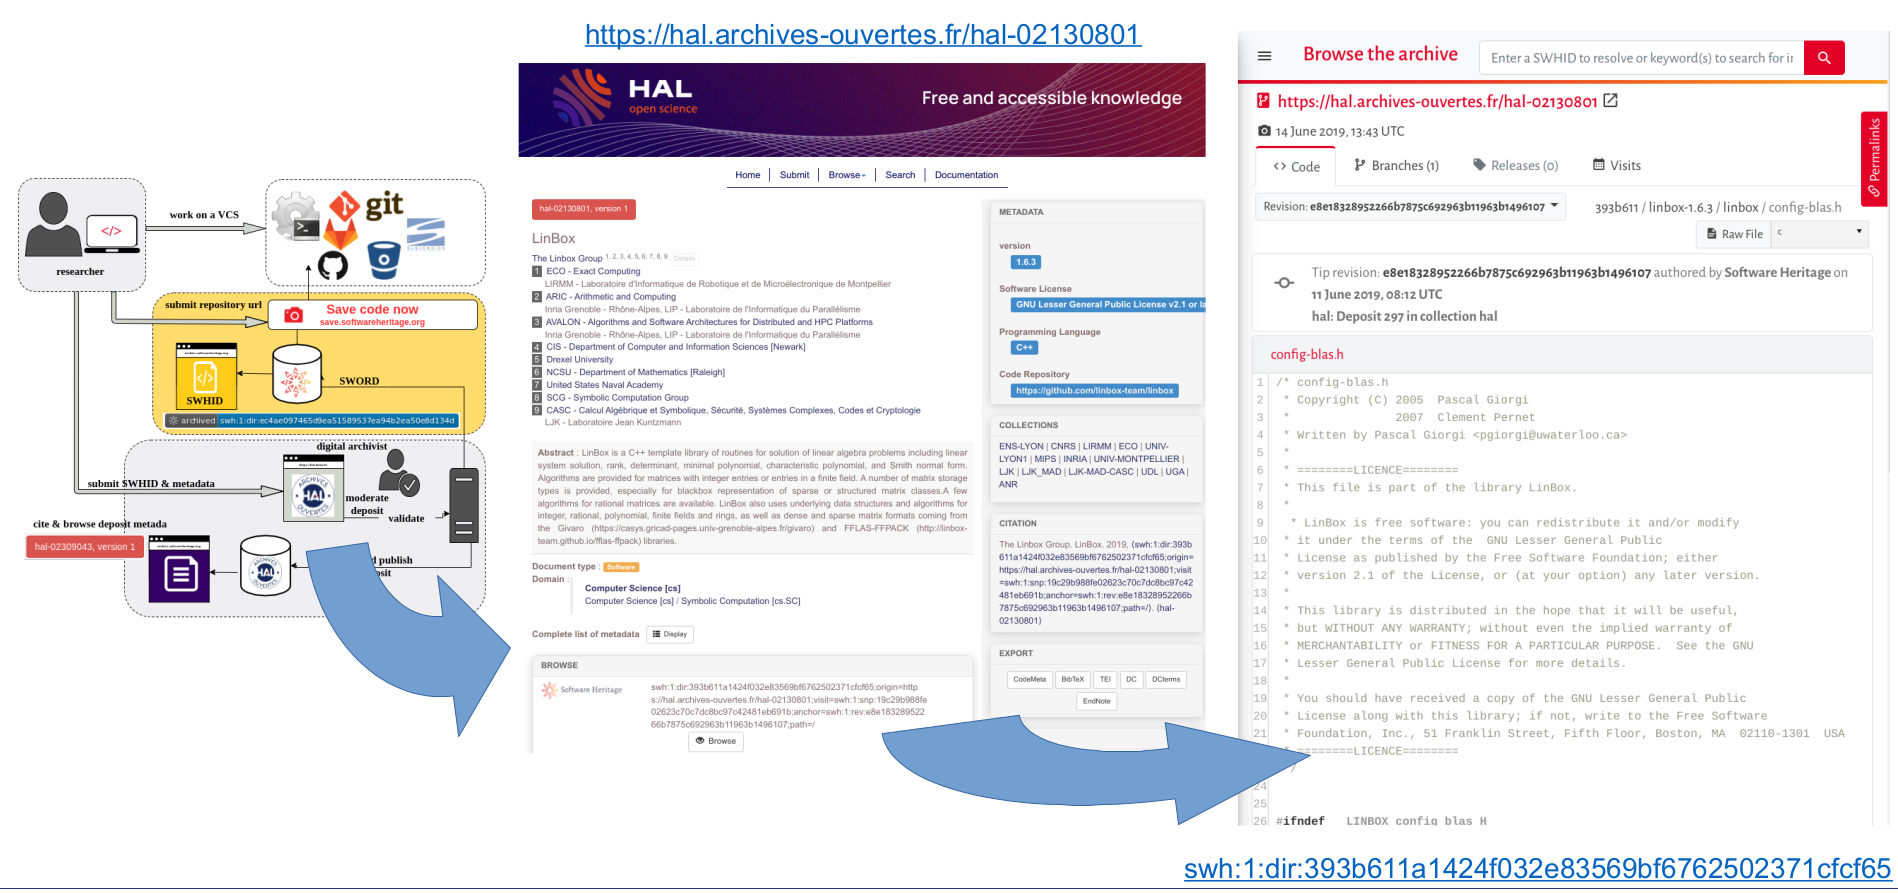
\includegraphics[width=.92\linewidth]{figures/hal-swh-overview.png}
  \caption[HAL and Software Heritage]{The HAL\,/\,Software Heritage synergy: a researcher deposits a
  curated record of a piece of software in the HAL open-access portal, while the source code itself
  is archived in Software Heritage --- the two linked by the code's \textsc{swhid}.}
  \label{fig:hal-swh}
\end{figure}

\begin{handson}[Hands-on: describe, and watch the citation appear]
Create a \texttt{codemeta.json} with the CodeMeta Generator, commit it, and re-archive the
repository. Then open the project in the Software Heritage archive and watch the citation panel
populate from your metadata --- and use it to produce the citation you actually want.
\end{handson}

\section{Cite and credit}

Finally, cite software as you would cite anything else in research: in the bibliography, as a
first-class reference. For decades there was no proper way to do this, and software citations were
forced into \texttt{@misc} entries that lost the version, the licence, and any verifiable
identifier~\autocite{2020GtCitation}. The \texttt{biblatex-software} style fixes
that~\autocite{DiCosmoSEN2020}. It adds four entry types --- \texttt{@software} for a project,
\texttt{@softwareversion} for a release, \texttt{@softwaremodule} for a component, and
\texttt{@codefragment} for a precise span of code --- chained with \texttt{crossref} so shared
metadata is written once, and, decisively, it carries a \texttt{swhid=} field. The package is on
CTAN and in TeX\,Live, and has shipped in the ACM \texttt{acmart} class since 2022, so the
\textsc{swhid} renders natively in an ACM paper (Figure~\ref{fig:biblatex-swh}).

\begin{figure}[htbp]
  \centering
  
\includegraphics[width=.9\linewidth]{figures/BibLaTeX-swh.png}
  \caption[Software in a bibliography, done right]{A software bibliography typeset with
  \texttt{biblatex-software}: each entry carries its version, licence, repository, and ---
  decisively --- a \textsc{swhid}, so the citation still resolves to the exact code long after the
  project's URL has rotted.}
  \label{fig:biblatex-swh}
\end{figure}

The payoff is that a software citation becomes \emph{reproducible}: a \textsc{swhid} in the
bibliography resolves to the exact bytes you used, with no dependence on a URL that may not outlive
the paper. This note's own bibliography is built this way --- the Parmap library, for instance, is
cited as a versioned software entry carrying its \textsc{swhid}, and a routine within it as a code
fragment.\footnote{See the \texttt{biblatex-software} entries~\autocite{parmap-1.1.1,simplemapper}
in the references.}

\takeaway{A \textsc{swhid} in the bibliography is a citation that still resolves when the URL is
gone.}

\begin{handson}[Hands-on: cite software with biblatex-software]
\begin{enumerate}[nosep,leftmargin=*]
  \item Write a \texttt{@softwareversion} entry for the code you archived, with its \texttt{swhid=}
        field; add a \texttt{@codefragment} child via \texttt{crossref} for a specific routine.
  \item Produce the variants --- a project-level \texttt{@software}, a \texttt{@softwaremodule} ---
        and compare how each renders.
  \item Drop the entries into an \texttt{acmart} article and confirm the \textsc{swhid} renders in
        the ACM template.
\end{enumerate}
\end{handson}

That is \textsc{ardc}: archive the code, reference it precisely, describe it, and cite it --- a
practice you can adopt incrementally, starting, as we keep saying because it is true, with your next
paper. The remaining question is what all this rigour \emph{buys} us. The answer, and the sharpest
test of the whole approach, is reproducibility and the evaluation of research artifacts: the
subject of the next chapter.

\chapter{Reproducibility and artifact evaluation}
\label{ch:repro}

How much of computational science can actually be re-run? It is an uncomfortable question, and the
honest answers are sobering --- which is why our community has built a process to force the issue:
\emph{artifact evaluation}, now standard at computer-science conferences, checks that the software
behind a paper actually exists, runs, and supports its claims. It is the sharpest test of
everything this note has argued for, and it turns out that Software Heritage answers its central
need almost perfectly. \textsc{ardc}, in other words, was the preparation; this chapter is the exam.

\takeaway{Artifact evaluation is the question this whole note was answering.}

\section{The reproducibility crisis}

The motivation is uncomfortable. When Collberg and Proebsting went looking for the code behind
several hundred papers from top computer-systems conferences, they found that, for a large majority,
the code could not be obtained, or could not be built~\autocite{Collberg2016}. Not refuted ---
simply \emph{unavailable}, or unbuildable, and so impossible to check at all. You cannot reproduce
what you cannot run; and, as the free-software tradition has always insisted, you cannot truly
inspect what you cannot read. A result resting on code is only as solid as our ability to get
\emph{that} code, at \emph{that} version, and run it again --- the gold standard being a
\emph{reproducible build} that yields, bit for bit, the same artifact from the same
source.\footnote{\url{https://reproducible-builds.org/}} The whole apparatus of artifact evaluation
exists to push back against this state of affairs.

\section{Artifact evaluation and badging}

Artifact evaluation began, fittingly, as a contest: at ESEC/FSE 2011, where the first prize went to
Vouillon and Di Cosmo. What started as an experiment is now a near-universal standard, codified by
the ACM \emph{Artifact Review and Badging} policy~\autocite{acmbadging}, which defines three
independent families of badge (Figure~\ref{fig:badges}):

\begin{description}[leftmargin=!,labelwidth=3.6cm,font=\bfseries\sffamily]
  \item[Artifacts Available] the artifacts are placed in a publicly accessible archival repository,
        with a unique identifier.
  \item[Artifacts Evaluated] the artifacts are documented, consistent, complete, and exercisable
        (\emph{Functional}) --- and, a notch higher, structured carefully for reuse
        (\emph{Reusable}).
  \item[Results Reproduced] the paper's results were independently obtained by others, with the
        authors' artifacts (\emph{Reproduced}) or without them (\emph{Replicated}).
\end{description}

\begin{figure}[htbp]
  \centering
  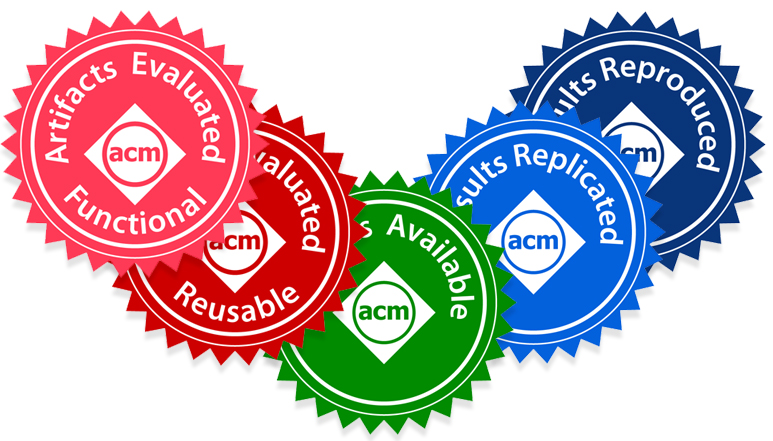
\includegraphics[width=.68\linewidth]{figures/acm-artifact-badges.png}
  \caption[The ACM artifact badges]{The ACM \emph{Artifact Review and Badging} badges. The
  \emph{Artifacts Available} badge --- a public archival repository plus a unique identifier --- is
  the one Software Heritage satisfies most literally.}
  \label{fig:badges}
\end{figure}

The practice has swept the field --- programming languages, software engineering, systems, security,
databases, high-performance computing --- to the point of routine: at EuroSys 2025 some 93\% of
papers earned the \emph{Functional} badge, and nearly half pursued \emph{Results Reproduced}. And it
is spreading beyond computer science: the AEA Data Editor now mandates a code-and-data audit for the
economics journals, initiatives such as CodeCheck and ReScience C independently re-run published
code, and NISO has generalised the whole badging scheme across the sciences~\autocite{nisorp31}.

\section{Artifact evaluation with Software Heritage}

Look again at the first badge. \emph{Artifacts Available} asks for two things: a publicly accessible
archival repository, and a unique identifier for the object. For decades this has been met by the
legacy recipe --- a zip deposited on Zenodo, figshare, or in the ACM Digital Library, with a DOI. We
have already seen, at length, why that recipe is weak for \emph{source code}: a DOI certifies a
landing page rather than the bytes (Chapter~\ref{ch:identifiers}); the deposit can change, carries no
granularity, and discards the development history (Chapter~\ref{ch:foundations}). Everything the
badge really wants --- a durable archive and a unique, verifiable name --- is exactly what
\textsc{ardc} delivers: archive the living repository in Software Heritage, and reference it with a
\textsc{swhid}.

This is not a departure from policy; it is the rigorous way to follow it. Software Heritage is
already among the archives ACM accepts for the \emph{Available} badge, the \textsc{swhid} is now
ISO/IEC 18670, and the software-engineering community has explicitly asked that it be used for
artifact evaluation~\autocite{sigsoftaecsoftware2022,isoiec18670}. The gain is sharpest for the
\emph{reviewer}. A DOI gives a reviewer a link to follow and a record to trust; a \textsc{swhid}
gives something a DOI never can --- the ability to \emph{recompute the identifier from the bytes
under review and check that it matches}, offline, in under a minute. If it matches, the reviewer
holds cryptographic proof that the artifact in hand is exactly the artifact the authors named. If it
does not, that too is a finding.

\begin{handson}[Hands-on: verify an artifact as a reviewer]
You are handed an artifact and the \textsc{swhid} the authors published for it.
\begin{enumerate}[nosep,leftmargin=*]
  \item Verify a file against its claimed content \textsc{swhid}: \texttt{swhid verify file.c
        swh:1:cnt:<hex>} --- it exits 0 only if the bytes match (Appendix~\ref{app:swhid-tools}).
  \item Re-compute the directory \textsc{swhid} of the whole artifact tree and compare it with the
        one in the paper. No archive, no network, and no trust required.
\end{enumerate}
\end{handson}

For the \emph{organiser}, the move is equally small: name Software Heritage in the call for
artifacts, and ask authors to put the qualified \textsc{swhid} of the precise artifact in the paper.
Each badge then maps cleanly onto a SWH-native check:

\begin{table}[htbp]
  \centering\small
  \begin{tabularx}{\linewidth}{@{}lX@{}}
    \toprule
    \textbf{ACM badge} & \textbf{Software Heritage--native check} \\
    \midrule
    Artifacts Available     & archived in Software Heritage; a qualified \textsc{swhid} in the paper \\
    Evaluated --- Functional & the reviewer fetches the \emph{exact} SWHID-pinned tree; no ``which zip?'' \\
    Evaluated --- Reusable   & \texttt{codemeta.json} + \texttt{CITATION.cff} + an \textsc{spdx} licence, under that \textsc{swhid} \\
    Results Reproduced      & reproduction starts from a verifiable, immutable identifier \\
    \bottomrule
  \end{tabularx}
  \caption[Badges mapped to SWH checks]{Each ACM badge mapped onto its Software Heritage--native check.}
  \label{tab:badge-crosswalk}
\end{table}

\takeaway{A reviewer can verify a \textsc{swhid} offline in a minute --- a DOI offers nothing of the
kind.}

\section{Double-blind review, and dense pinpointing}

Artifact evaluation often happens under \emph{double-blind} review, which seems to pose a problem:
how do you share your code without revealing who wrote it? Tools that rewrite a repository's history
to anonymise it are fragile, and they leak. The intrinsic identifier sidesteps the whole difficulty.
A \emph{directory} \textsc{swhid} is computed from content alone --- no author, no origin, no commit
metadata, nothing to scrub --- and it works for any technology, not just Git. Submit the
\texttt{dir} \textsc{swhid}; reviewers confirm the bytes are exactly yours while learning nothing
about you.

The same idea scales to a paper that pinpoints code throughout its body. Modern papers already do
this densely: \emph{Source Code Hotspots} ties its findings to exact passages, naming each with a
qualified \textsc{swhid} so a reader can open the precise lines in the
archive~\autocite{spinellis2026hotspots}. And the part that carries \emph{provenance} is precisely
the qualifiers --- \texttt{origin}, \texttt{visit}, \texttt{anchor} --- while the core hash, the
identifier proper, reveals nothing about authorship. So the \emph{only} difference between the double-blind
submission and the camera-ready version is removing, then restoring, those qualifiers: the core
hashes are identical, and every pinpoint a reviewer checked during blind review stays valid, to the
character, in the final paper. One mechanical, fully reversible edit --- no history-rewriting, no
risk of a leak.

\takeaway{Double-blind vs camera-ready: strip, then restore, the qualifiers --- the content hash
never changes.}

\begin{handson}[Hands-on: a double-blind artifact]
Compute the directory \textsc{swhid} of your artifact tree (\texttt{swhid dir ./}; see
Appendix~\ref{app:swhid-tools}) and submit \emph{that}. It names your exact bytes and nothing else.
After acceptance, archive the repository and add the \texttt{origin}/\texttt{anchor} qualifiers ---
the same identifier, now pointing home.
\end{handson}

\section{Built into the record of science}

Best of all is when none of this is left to the author's goodwill. Since November 2020 the journal
\emph{eLife} has archived the code behind every article in Software Heritage automatically, embedding
the \textsc{swhid} in the article's machine-readable metadata and validating it before
publication~\autocite{elifeswh2020}. Availability stops being a promise a reviewer checks once, and
becomes a durable property of the published record itself --- which is, in the end, exactly where it
belongs.

That is the case for building artifact evaluation on Software Heritage. What remains is to look
outward: at how widely this is already being adopted, the policy that now backs it, and the larger
mission it serves. That is the final chapter.

\chapter{Adoption, policy and outlook}
\label{ch:outlook}

\begin{objectives}\small
\begin{itemize}[nosep,leftmargin=*]
  \item survey where this practice is already adopted, and the policy that backs it;
  \item situate Software Heritage in the resilience, sovereignty, and transparent-AI agendas;
  \item identify what to do as a researcher, a reviewer, or an institution.
\end{itemize}
\end{objectives}

We have built the argument and shown the practice. It remains to look outward: to see that this is
already happening, that policy now stands behind it, and that the same infrastructure serves a
mission far larger than open science. And then to ask what you can do, starting --- one last time
--- with your next paper.

\takeaway{Open science is one payoff of software preservation; resilience, transparency, and
sovereignty are others.}

\section{It is already happening}

None of this is hypothetical. Journals and platforms across disciplines have wired Software Heritage
into how they work: the HAL national repository offers a curated software-deposit workflow; IPOL
publishes image-processing papers with runnable code and a SWHID; \emph{eLife} archives the code
behind every article automatically; \emph{swMATH} references mathematical software in the archive;
and Episciences journals such as JTCAM ask authors to cite their software with
\texttt{biblatex-software} (itself shipped in the ACM article class since
2022)~\autocite{SwhCACM2018}. The connections keep multiplying: Episciences now links each published
article to its code through a \textsc{swhid}~\autocite{episciences2025swh}; \emph{Zenodo} forwards
its software deposits to the archive (Chapter~\ref{ch:ardc}); and code-publishing venues such as
Dagstuhl's \emph{DROPS} interconnect the same way.\footnote{\url{https://drops.dagstuhl.de/}.} Papers
themselves now carry not one identifier but many, pinpointing their code passages with qualified
\textsc{swhid}s throughout the text~\autocite{spinellis2026hotspots}.

And the stakes are real, not niche. When the French ministry surveyed its research-software
producers, the picture that emerged was of long-lived, widely-used, high-impact work: half of the
software reported was more than nine years old, a third had over a hundred users, and nearly
two-thirds had impact beyond academia --- overwhelmingly released as free and open
source.\footnote{French Ministry of Higher Education and Research, research-software survey, 2023.}
This is not a fringe of scientific practice; it is a load-bearing part of it, and it has been going
uncared-for.

\section{The policy that backs it}

The direction of travel, at every level, is now unambiguous. The \textbf{UNESCO Recommendation on
Open Science} (2021) calls for source code to be released openly, and for open-science
infrastructures to be \enquote{organized and financed upon an essentially not-for-profit and
long-term vision}~\autocite{UNESCO2021OpenScience}. The European \textbf{EOSC SIRS report} (2020) is
more specific still: \emph{archive in Software Heritage, use the SWHID}, and treat open source as the
default for research software, with deviations to be justified~\autocite{SIRSReport2020}. The
\textbf{Paris Call on Software Source Code} (2019) had already urged the world to \enquote{recognise
software source code as a fundamental enabler in all aspects of human endeavour} and to build shared
infrastructures to preserve it~\autocite{ParisCall2019}. And at the national level the message is the
same: France's second \textbf{National Plan for Open Science} names Software Heritage and the
\textsc{swhid} explicitly, the country's research-infrastructure roadmap now lists the archive, and a
standing College for research software carries the agenda forward~\autocite{PNSO2_2021,osec_2022}.
Strip away the acronyms and a single instruction remains: archive in Software Heritage, and identify
with a \textsc{swhid}.

\begin{figure}[htbp]
  \centering
  
\includegraphics[height=5.3cm]{figures/EOSC-SIRS-report.png}\hspace{7mm}
  
\includegraphics[height=5.3cm]{figures/PNSO2-en-cover.png}
  \caption[Policy documents]{Two of the documents that now point research software at Software
  Heritage: the EOSC \emph{Scholarly Infrastructures for Research Software} report (left,
  2020)~\autocite{SIRSReport2020} and France's second National Plan for Open Science (right,
  2021--2024)~\autocite{PNSO2_2021}.}
  \label{fig:policy}
\end{figure}

Funders have followed. France's national research agency, the ANR, asks in its own funding
guidelines that project software be released under a libre licence and its source archived in
Software Heritage, with the grant referenced (Figure~\ref{fig:anr}).

\begin{figure}[htbp]
  \centering
  \fbox{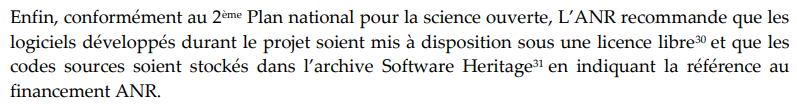
\includegraphics[width=.96\linewidth]{figures/anr-recommendations.png}}
  \caption[ANR funding guideline]{From the ANR's funding guidelines: project source code is to be
  stored in Software Heritage under a free licence, with the ANR grant referenced.}
  \label{fig:anr}
\end{figure}

\takeaway{The policy is unambiguous: archive in Software Heritage, identify with a \textsc{swhid}.}

\section{The wider mission: resilience, sovereignty, transparent AI}

Open science is only one of the things this archive makes possible, and stepping back reveals why it
matters beyond the library. The same uniform record of the world's source code is the foundation for
several urgent agendas at once. It underpins \emph{software supply-chain traceability}: an
intrinsic identifier is exactly what a software bill of materials (an \textsc{sbom}) needs, and what
regulators reaching for the EU Cyber Resilience Act will
require~\autocite{EU_CRA_2024,barais2025swhidcyber}. It underpins
\emph{transparent AI}: the very large code corpora that train today's models --- The Stack, on which
StarCoder is built --- are drawn from Software Heritage, and provenance for that data is becoming a
legal as well as an ethical demand~\autocite{StarCoder2_2024}. And it underpins \emph{resilience}:
because the archive holds the code with its history, a build system can fall back to it when the
upstream platform fails. Guix has done exactly this since 2019 --- when a package vanishes from its
registry, the build continues from Software Heritage~\autocite{dicosmo_tpdl_2022,SWHecosystems2023}.
The point is not academic. If GitHub or PyPI disappeared tomorrow, much of the digital world would
not merely slow down --- it would stop.

This reframes the whole enterprise. The goal is not to \emph{own} the infrastructure but to ensure
that nothing essential can vanish --- a shared, open, non-rival archive that benefits all while
leaving each free to build on it. That is digital sovereignty rightly understood: not autarky, but
\emph{resilience}.

\section{A fair question: what about Software Heritage itself?}

This note has argued that platforms fail and that we should plan for it --- so it must turn the same
lens on the archive it recommends. Software Heritage is a non-profit initiative launched in 2016,
hosted by Inria and run as an international, multi-stakeholder effort under an agreement with UNESCO;
it is funded by a range of institutional members and sponsors rather than by any single company or
state, with foundational support from bodies such as the Alfred P.\ Sloan and NLnet foundations. Its
answer to its own single-point-of-failure risk is a \emph{network of independent mirrors} --- full
copies of the archive held by partner institutions, so the corpus survives the loss of any one
operator. It is the same resilience-by-redundancy the archive offers your build chain, turned on
itself. For an editor or a funder weighing a ten-year commitment, that --- not a metaphor --- is the
due-diligence answer.

It is equally worth being clear about the \emph{limits}. A \textsc{swhid} secures the \emph{identity}
and \emph{availability} of source code; it does not make a build deterministic
(Chapter~\ref{ch:repro}), and it cannot open code that was never public. Adoption, though real and
growing, is still offered as one option among several at most venues rather than a default. The
claim of this note is not that the work is finished --- it is that the infrastructure, the standard,
and the practice are now ready to be made the default.

\section{Call to action}

Which brings us, finally, back to you. The tools are built, the policy is written, the adoption is
under way; the one thing still missing is the habit. So make it, at three scales.

\emph{As a researcher:} archive the code behind your next result in Software Heritage, reference it
with a \textsc{swhid} at the granularity your claim needs, describe it, and cite it. That is the
whole of \textsc{ardc}, and you can do it this week.

\emph{As a reviewer, an editor, or a member of an artifact-evaluation committee:} ask authors for
archival proof --- a \textsc{swhid} --- rather than a fragile URL. It is one small habit, but applied
every time, it changes the norms of a whole community.

\emph{As an institution or a funder:} write Software Heritage into your open-science policy, become a
member or run a mirror, and --- not least --- count high-quality software contributions in the
careers of the people who make them.

\begin{callout}{Ready to paste: a grant condition and a policy line}
\small \textbf{Grant condition} (it costs the grantee nothing --- archival is free):
\begin{quote}\itshape
Source code produced with this grant must be released under an open licence and archived in Software
Heritage, and the resulting \textsc{swhid} reported in the project's outputs. (Further documentation,
testing, and packaging are encouraged but not required.)
\end{quote}
\textbf{Open-science / sovereignty policy line:}
\begin{quote}\itshape
We adopt intrinsic, standard identifiers (\textsc{swhid}, ISO/IEC~18670) and a shared, non-profit
archive (Software Heritage) for research software, ensuring that publicly funded code remains
verifiable, citable, and recoverable independently of any commercial platform.
\end{quote}
A funder can audit compliance across a whole portfolio with one HAL-API call
(\S\,\ref{ch:ardc}'s \texttt{collCode\_s} query), no per-project chasing required.
\end{callout}

Software source code is a precious, unique form of knowledge, and for too long we have treated it as
an afterthought. We no longer have to. The argument is settled and the machinery is ready; what is
needed now is simply that we use it. Record your code, share it, and value
it~\autocite{NatureSD2026}. Start with your next paper.


% --- Appendices ----------------------------------------------------------
\appendix
\setchapvignette[6cm]{appendix-cookbook}
\chapter{Command cookbook}
\label{app:cookbook}

There are two interchangeable local toolchains for computing and checking \textsc{swhid}s, and
they produce the \emph{same} identifiers for the same bytes --- pick whichever suits your
environment. \textbf{Path~A} is \texttt{swhid-rs}, the Rust reference implementation of the
standard (ISO/IEC~18670, MIT license): fast, standalone, and the one that tracks the specification
most closely. \textbf{Path~B} is the original Python implementation --- \texttt{swh identify}
(from \texttt{swh.model}) and \texttt{swh scanner} --- which adds two things the Rust CLI does not
yet cover: snapshot identifiers, and scanning a working tree against the archive. Appendix~%
\ref{app:swhid-tools} compares all the implementations in full. The two paths below mirror each
other operation for operation; the shared section at the end is the same whichever you chose.

\paragraph{Path A --- the Rust reference tool (\texttt{swhid-rs}).}
\begin{verbatim}
# --- Install -------------------------------------------------------------
cargo install swhid                  # swhid-rs (Rust reference impl., MIT)
cargo install swhid --features git   # ...with VCS (revision) support
# or download a pre-built binary from the project's releases page:
#   https://github.com/swhid/swhid-rs

# --- Compute core SWHIDs locally ----------------------------------------
swhid content --file file.c          # -> swh:1:cnt:...
swhid dir src/                 # -> swh:1:dir:...  (Merkle hash of tree)
swhid parse "swh:1:cnt:<hex>"        # validate / pretty-print a SWHID

# A revision SWHID is just the git commit hash:
echo "swh:1:rev:$(git rev-parse HEAD)"     # -> swh:1:rev:...

# --- Verify bytes against a claimed SWHID (exit 0 iff they match) --------
swhid verify file.c swh:1:cnt:<hex>        # PATH first, then SWHID
swhid verify src/   swh:1:dir:<hex>

# Snapshot SWHIDs and tree scanning: use Path B below.
\end{verbatim}

\paragraph{Path B --- the Python tools (\texttt{swh.model} + \texttt{swh.scanner}).}
\begin{verbatim}
# --- Install -------------------------------------------------------------
pip install 'swh.model[cli]'         # swh identify
pip install swh.scanner              # swh scanner

# --- Compute SWHIDs locally (auto-detects type, or force with --type) ---
swh identify file.c                  # -> swh:1:cnt:...
swh identify --type directory src/   # -> swh:1:dir:...
swh identify --type directory ./export/    # a CLEAN export -> swh:1:dir:...
#   (never a live checkout: see the caveat below)
swh identify --type snapshot repo.git/     # -> swh:1:snp:...  (snapshot)

# --- Verify bytes against a claimed SWHID (exit 0 iff they match) --------
swh identify --verify swh:1:cnt:<hex> file.c    # SWHID first, then PATH

# --- Scan a working tree against the archive ----------------------------
swh scanner scan ./repo                    # what is already archived?
\end{verbatim}

\paragraph{Shared --- archive and resolve (no install needed).}
\begin{verbatim}
# Archive a public repo:  https://save.softwareheritage.org
# Resolve any SWHID:      https://archive.softwareheritage.org/<swhid>
\end{verbatim}

\noindent\textbf{One caveat for \texttt{dir} hashes.} A directory \textsc{swhid} is computed over
everything below the directory you point the tool at --- including a \texttt{.git/} directory,
build output and editor droppings --- and it depends on file \emph{permissions} as well as
content. To match what the archive stored from a git repository, never hash a live checkout:
compute over a clean export (\texttt{git archive} unpacked into an empty directory), whose hash
equals \verb|git rev-parse <commit>^{tree}| by construction. If a directory check mismatches
where a content check would pass, suspect a polluted working copy first, and permission bits
second.

\chapter{SWHID syntax cheat-sheet}
\label{app:swhid-syntax}

This appendix summarises the \textsc{swhid} grammar. It is \emph{not} normative: the authority is
the \emph{SWHID Specification, version 1.2}~\autocite{swhidspec}, published openly on
swhid.org and standardised, word for word, as ISO/IEC~18670:2025~\autocite{isoiec18670}. The
section pointers below refer to that specification.

\section{Core identifiers (spec \S5)}

A \emph{core} \textsc{swhid} is four colon-separated fields,
\swhid{swh:1:\textit{type}:\textit{hash}}\,:\footnote{\url{https://www.swhid.org/specification/v1.2/5.Core_identifiers/}}
the scheme \texttt{swh}; the schema version (\texttt{1}); a three-letter object \emph{type}; and a
40-digit, lowercase-hex object \emph{identifier}. That identifier is a \textsc{sha}-1 computed over a
git-style serialisation of the object --- so a revision \textsc{swhid} is exactly the Git commit
hash with \texttt{swh:1:rev:} prepended. The five types are:

\begin{table}[htbp]
  \centering\small
  \begin{tabularx}{\linewidth}{@{}llX@{}}
    \toprule
    \textbf{Code} & \textbf{Object} & \textbf{Identifies} \\
    \midrule
    \texttt{cnt} & content   & the bytes of a single file \\
    \texttt{dir} & directory & a directory tree (names, permissions, and child hashes) \\
    \texttt{rev} & revision  & a commit, with its parents, author, and date \\
    \texttt{rel} & release   & a named release (annotated tag) \\
    \texttt{snp} & snapshot  & a repository's full state at one visit (all branches and tags) \\
    \bottomrule
  \end{tabularx}
\end{table}

\section{Qualified identifiers (spec \S6)}

A \emph{qualified} \textsc{swhid} appends a sequence of qualifiers to a core identifier, each
introduced by \texttt{;} and written \texttt{name=value}.\footnote{\url{https://www.swhid.org/specification/v1.2/6.Qualified_identifiers/}}
The core \emph{identifies}; the qualifiers \emph{locate} and \emph{contextualise}.

\begin{table}[htbp]
  \centering\small
  \begin{tabularx}{\linewidth}{@{}llX@{}}
    \toprule
    \textbf{Qualifier} & \textbf{Kind} & \textbf{Meaning} \\
    \midrule
    \texttt{origin} & context  & the URI the code was harvested from \\
    \texttt{visit}  & context  & the snapshot \textsc{swhid} of the visit \\
    \texttt{anchor} & context  & a node (\texttt{dir}/\texttt{rev}/\texttt{rel}/\texttt{snp}) the \texttt{path} is rooted at \\
    \texttt{path}   & context  & an absolute path from the anchor's root directory \\
    \texttt{lines}  & fragment & a line range within a \texttt{cnt} (1-based, inclusive; \texttt{A} or \texttt{A-B}) \\
    \texttt{bytes}  & fragment & a byte range within a \texttt{cnt} (0-based, inclusive) \\
    \bottomrule
  \end{tabularx}
\end{table}

The rules (spec \S6): each qualifier appears at most once; \texttt{visit} requires \texttt{origin};
\texttt{anchor} requires \texttt{path}; and the fragment qualifiers \texttt{lines}/\texttt{bytes}
apply only to a \texttt{cnt}. The recommended order is \texttt{origin}, \texttt{visit},
\texttt{anchor}, \texttt{path}, then \texttt{lines} or \texttt{bytes}.

\section{A worked example}

The specification's own example pins lines 9--15 of one file, in one revision, of one archived
repository:

\begin{verbatim}
swh:1:cnt:4d99d2d18326621ccdd70f5ea66c2e2ac236ad8b;
  origin=https://gitorious.org/ocamlp3l/ocamlp3l_cvs.git;
  visit=swh:1:snp:d7f1b9eb7ccb596c2622c4780febaa02549830f9;
  anchor=swh:1:rev:2db189928c94d62a3b4757b3eec68f0a4d4113f0;
  path=/Examples/SimpleFarm/simplefarm.ml;
  lines=9-15
\end{verbatim}

\noindent(written on a single line in practice). To compute or verify a \textsc{swhid}, see
Appendix~\ref{app:swhid-tools}.

\chapter{Glossary}
\label{app:glossary}

% TODO: flesh out definitions.
\begin{description}[leftmargin=!,labelwidth=2.6cm,font=\bfseries]
  \item[ARDC] Archive, Reference, Describe, Cite \& credit --- the four needs for research
        software.
  \item[SWHID] SoftWare Hash IDentifier; an intrinsic identifier (ISO/IEC~18670:2025).
  \item[Core SWHID] \swhid{swh:1:<type>:<hash>}; the content fingerprint.
  \item[Qualified SWHID] a core \textsc{swhid} plus \texttt{origin}/\texttt{visit}/%
        \texttt{anchor}/\texttt{path}/\texttt{lines} qualifiers.
  \item[Origin] the URL where the code was found (a \texttt{visit} target).
  \item[Snapshot] the full state of a repository at one visit (\texttt{snp}).
  \item[Forge] a development platform (GitHub, GitLab, \dots) --- \emph{not} an archive.
  \item[Intrinsic identifier] computed from the content; verifiable offline, no registry.
\end{description}

\chapter{SWHID tool implementations}
\label{app:swhid-tools}

A \textsc{swhid} is, by design, something anyone can compute: the whole point of an intrinsic
identifier is that it owes nothing to a registry, so a name you can only obtain from a central
service would betray the idea. Now that the \textsc{swhid} is an international standard
(ISO/IEC~18670:2025), a small ecosystem of independent implementations has grown up around it ---
in several languages, at several levels of ambition --- and they all compute, for the same bytes,
the same name. That is the standard doing its job.

For everyday work you need only two of them. The \emph{reference implementation} is
\texttt{swhid-rs}, written in Rust and released under the \textsc{mit} licence; it tracks the ISO
specification directly and is the tool this note reaches for first. The Python
\texttt{swh.model} package (the \texttt{swh identify} command) remains the most complete in
coverage --- snapshots, deposits, the full archive toolchain --- and \texttt{swh scanner} answers
the complementary question of \emph{what the archive already holds}. The rest of the table records
the alternatives you may meet in the wild, and the no-install resolvers that turn a \textsc{swhid}
back into the code it names.

\begingroup
\small
\setlength{\extrarowheight}{2pt}
\begin{table}[htbp]
  \centering
  \caption[SWHID tool implementations]{Implementations and resolvers for the \textsc{swhid}
  standard (ISO/IEC~18670). The Rust tool \texttt{swhid-rs} is the reference implementation; the
  Python \texttt{swh.model} CLI is the most feature-complete. Resolvers need no installation at
  all.}
  \label{tab:swhid-tools}
  \begin{tabularx}{\linewidth}{@{}>{\raggedright\arraybackslash}p{2.5cm}%
                                  >{\raggedright\arraybackslash}p{2.0cm}%
                                  >{\raggedright\arraybackslash}X@{}}
    \toprule
    \textbf{Name} & \textbf{Language /\newline ecosystem} & \textbf{What it does \& how to use it} \\
    \midrule
    \texttt{swhid-rs}
      & Rust \newline (\textsc{mit})
      & \emph{Reference implementation} of ISO/IEC~18670. Computes and verifies core
        \textsc{swhid}{s}. \texttt{cargo install swhid} (add \texttt{-{}-features git} for
        revision support), or grab a pre-built binary from the releases page.
        \texttt{swhid content -{}-file F}, \texttt{swhid dir DIR}, \texttt{swhid verify PATH SWHID},
        \texttt{swhid parse "swh:1:\textellipsis"}.
        \scriptsize\url{https://github.com/swhid/swhid-rs} \\
    \addlinespace
    \texttt{swh.model} \newline (\texttt{swh identify})
      & Python
      & The most complete CLI: content, directory, revision \emph{and} snapshot identifiers, plus
        \texttt{-{}-verify}. \texttt{pip install 'swh.model[cli]'}, then e.g.\
        \texttt{swh identify -{}-type snapshot repo.git/}.
        \scriptsize\url{https://gitlab.softwareheritage.org/swh/devel/swh-model} \\
    \addlinespace
    \texttt{swh scanner}
      & Python
      & Walks a working tree and tells you which files and directories are \emph{already archived}
        in Software Heritage --- the complement to computing a name.
        \texttt{pip install swh.scanner}; \texttt{swh scanner scan ./repo}.
        \scriptsize\url{https://gitlab.softwareheritage.org/swh/devel/swh-scanner} \\
    \addlinespace
    \emph{updateswh} \newline (Permalinks)
      & Browser \newline extension
      & The point-and-click route: a button on GitHub / GitLab / Bitbucket pages that triggers
        archival and then exposes the artifact's \textsc{swhid} via the archive's \emph{Permalinks}
        tab. No local install of a hashing tool needed.
        \scriptsize\url{https://www.softwareheritage.org/browser-extensions/} \\
    \addlinespace
    Archive \& \texttt{n2t.org} resolvers
      & Web service \newline (no install)
      & Turn a \textsc{swhid} \emph{back} into code: paste it after
        \texttt{https://archive.softwareheritage.org/} to browse the bytes, or resolve via the
        \texttt{n2t.org} name-resolver (\texttt{https://n2t.net/}).
        \scriptsize\url{https://archive.softwareheritage.org/} \\
    \addlinespace
    \texttt{swhid} for OCaml
      & OCaml
      & A community library (OCamlPro) to parse, build and manipulate \textsc{swhid}{s}.
        \texttt{opam install swhid}.
        \scriptsize\url{https://github.com/OCamlPro/swhid} \\
    \addlinespace
    \texttt{swhid-go}, \texttt{swhid-ruby}
      & Go, Ruby
      & Independent ports of the standard for Go and Ruby toolchains.
        \scriptsize\url{https://github.com/andrew/swhid-go} \\
    \bottomrule
  \end{tabularx}
\end{table}
\endgroup

\noindent A practical rule of thumb: reach for \texttt{swhid-rs} when you want the
reference behaviour and a single fast binary; fall back to \texttt{swh identify} for snapshots and
the deeper archive workflow; and remember that for a one-off check you need install nothing at all
--- the resolver at \url{https://archive.softwareheritage.org/} will take any \textsc{swhid} and
hand you back the code it names.

\chapter{Policy reference: the instrument matrix}
\label{app:policy}

Policy is the part of an argument that ages fastest and scatters worst. Across
Chapter~\ref{ch:outlook} the instruments arrive one at a time, in the order the prose needs
them --- a UNESCO recommendation here, an EOSC report there, a French national plan a paragraph
later --- and that is the right way to make the case, but the wrong way to \emph{act} on it. A
reader who wants to write a clause, brief a funder, or check whether their own jurisdiction has
already moved should not have to reassemble the list from the body text; and a future drafter of
this note should not have to rediscover, each time, which mandate said exactly what.

\takeaway{One matrix, every instrument: jurisdiction, date, mandate, link --- the deduplicated
landing point for the policy that backs the practice.}

\noindent And so, here, deduplicated into a single matrix, is every policy instrument surfaced in
this note and in the inventories behind it. Read each row as a pointer, not a paraphrase: the
mandate column quotes the source \emph{verbatim} where a quotable line exists, and otherwise gives
the shortest faithful summary, with the citation and the live link carrying the rest. The list
leans European, and French in particular --- that is where the convergence happened first and
hardest --- but the international and national rows show that the direction of travel is the same
everywhere: open the code, preserve it, and name it intrinsically.

{\footnotesize
\setlength{\extrarowheight}{2pt}
\begin{longtable}{@{}>{\raggedright\arraybackslash}p{2.7cm}%
                    >{\raggedright\arraybackslash}p{2.15cm}%
                    >{\raggedright\arraybackslash}p{0.95cm}%
                    >{\raggedright\arraybackslash}p{1.15cm}%
                    >{\raggedright\arraybackslash}p{4.7cm}@{}}
\caption[Policy instrument matrix]{Deduplicated matrix of policy instruments pointing research
software at open licensing, preservation, and intrinsic identification. Mandates are quoted
verbatim where a quotable line exists; links resolve the full text.}\label{tab:policy}\\
\toprule
\textbf{Instrument} & \textbf{Issuing body} & \textbf{Juris.} & \textbf{Date} &
\textbf{Core mandate (verbatim where available)} \\
\midrule
\endfirsthead
\multicolumn{5}{l}{\footnotesize\itshape Table~\ref{tab:policy}, continued from previous page}\\
\toprule
\textbf{Instrument} & \textbf{Issuing body} & \textbf{Juris.} & \textbf{Date} &
\textbf{Core mandate} \\
\midrule
\endhead
\midrule
\multicolumn{5}{r}{\footnotesize\itshape continued on next page}\\
\endfoot
\bottomrule
\endlastfoot

% --- International ---------------------------------------------------------
\textbf{Rec.\ on access to research data from public funding}~\autocite{OECD2021ResearchData}%
  \newline\scriptsize\url{https://legalinstruments.oecd.org/en/instruments/OECD-LEGAL-0347}
  & OECD Council & Intl & 2006 (rev.\ 2021)
  & Access to, and re-use of, publicly funded research data as a default principle. \\
\addlinespace
\textbf{Paris Call on Software Source Code}~\autocite{ParisCall2019}%
  \newline\scriptsize\url{https://en.unesco.org/foss/paris-call-software-source-code}
  & UNESCO, Inria, Software Heritage & Global & Feb 2019
  & \enquote{recognise software source code as a fundamental enabler in all aspects of human
    endeavour}; build shared infrastructures to preserve it. \\
\addlinespace
\textbf{Recommendation on Open Science}~\autocite{UNESCO2021OpenScience}%
  \newline\scriptsize\url{https://unesdoc.unesco.org/ark:/48223/pf0000379949}
  & UNESCO & Global & 2021
  & Open science including open-source code: \enquote{source code must be included in the software
    release}. \\
\addlinespace[4pt]

% --- European Union -------------------------------------------------------
\textbf{Rec.\ 2018/790 on access to \& preservation of scientific information}~\autocite{ECRec2018_790}%
  \newline\scriptsize\url{https://eur-lex.europa.eu/eli/reco/2018/790/oj}
  & European Commission & EU & 25 Apr 2018
  & Open access to, and long-term preservation of, scientific information and the outputs of
    publicly funded research. \\
\addlinespace
\textbf{Directive 2019/790 (Copyright in the DSM)}~\autocite{EU_CopyrightDir2019}%
  \newline\scriptsize\url{https://eur-lex.europa.eu/eli/dir/2019/790/oj}
  & EU Parliament \& Council & EU & 2019
  & Copyright reform bearing on text-and-data mining and the legal status of source-code re-use. \\
\addlinespace
\textbf{EOSC SIRS report}~\autocite{SIRSReport2020}%
  \newline\scriptsize\url{https://data.europa.eu/doi/10.2777/28598}
  & EOSC Executive Board (EC) & EU & Dec 2020
  & Archive in Software Heritage, use the \textsc{swhid}; \enquote{all research software \textellipsis\
    Open Source license by default \textellipsis\ deviations \textellipsis\ properly motivated}. \\
\addlinespace
\textbf{Task Force on quality research software}~\autocite{EOSC_TaskForce2021}%
  \newline\scriptsize\url{https://eosc.eu/advisory-groups/infrastructures-quality-research-software/}
  & EOSC Association & EU & 2021
  & Recommendations for FAIR, open, and sustainable research software. \\
\addlinespace
\textbf{FAIRCORE4EOSC}~\autocite{FAIRCORE4EOSC2022}%
  \newline\scriptsize\url{https://faircore4eosc.eu/}
  & Horizon Europe consortium & EU & 2022
  & Builds core EOSC persistent-identifier and metadata components, with Software Heritage among the
    partners. \\
\addlinespace[4pt]

% --- France ---------------------------------------------------------------
\textbf{Loi pour une R\'epublique num\'erique (Loi Lemaire)}~\autocite{LoiLemaire2016}%
  \newline\scriptsize\url{https://www.legifrance.gouv.fr/loda/id/JORFTEXT000033202746}
  & R\'epublique fran\c{c}aise & France & Oct 2016
  & Open public data and the source code of administrations as a default. \\
\addlinespace
\textbf{PM circular on data, algorithms \& source code}~\autocite{PMdirective2021}%
  \newline\scriptsize\url{https://www.legifrance.gouv.fr/circulaire/id/45162}
  & Premier ministre & France & 27 Apr 2021
  & Public data, algorithms and source code open by default across the State. \\
\addlinespace
\textbf{2\textsuperscript{nd} National Plan for Open Science (PNSO2)}~\autocite{PNSO2_2021}%
  \newline\scriptsize\url{https://www.ouvrirlascience.fr/wp-content/uploads/2021/10/Second_French_Plan-for-Open-Science_web.pdf}
  & Minist\`ere de l'ESR & France & 6 Jul 2021
  & Names Software Heritage and the \textsc{swhid} explicitly; open-source research software by
    default. \\
\addlinespace
\textbf{Law 2022-217 (loi 3DS), art.\ 163}~\autocite{LoiArticle163_2022}%
  \newline\scriptsize\url{https://www.legifrance.gouv.fr/jorf/id/JORFTEXT000045197395}
  & R\'epublique fran\c{c}aise & France & 21 Feb 2022
  & 18-month report to Parliament on the production and valorization of public-research software
    (the 2023 \emph{Rapport Boulet}~\autocite{boulet2023etatdeslieux}). \\
\addlinespace[4pt]

% --- United States --------------------------------------------------------
\textbf{Executive Order 14028, \S4}~\autocite{USEO14028_2021}%
  \newline\scriptsize\url{https://www.federalregister.gov/d/2021-10460}
  & White House & US & 12 May 2021
  & Software supply-chain security; mandates a software bill of materials (\textsc{sbom}). \\
\addlinespace
\textbf{Scientific Information Policy (SPD-41a)}~\autocite{NASA_OSI_2022}%
  \newline\scriptsize\url{https://science.nasa.gov/researchers/science-information-policy/}
  & NASA & US & Dec 2022
  & Open code, data and publications by default for NASA-funded research. \\
\addlinespace[4pt]

% --- Germany --------------------------------------------------------------
\textbf{Model curriculum vitae}~\autocite{DFG_CV_2022}%
  \newline\scriptsize\url{https://www.dfg.de/en/research_funding/announcements_proposals/2022/info_wissenschaft_22_61}
  & DFG & Germany & Sept 2022
  & Recognises research software as a citable scholarly output in evaluation and CVs. \\

\end{longtable}}

\noindent A practical rule of thumb for reading the matrix: the \emph{global} rows (OECD, the Paris
Call, UNESCO) set the principle; the \emph{European} rows turn it into operational guidance ---
SIRS is the one to quote when someone asks for chapter and verse, because it names Software Heritage
and the \textsc{swhid} outright; and the \emph{national} rows are what a researcher or a funder
points to in their own jurisdiction. Strip the acronyms from any of them and the same instruction
remains, the one this whole note has been arguing for: open the code, preserve it, and identify it
with an intrinsic, standard name.


% --- References ----------------------------------------------------------
\printbibliography[heading=bibintoc,title={References}]

% --- Colophon: the note archives and verifies itself ---------------------
\clearpage
\chapter*{Colophon: archiving these notes}
\addcontentsline{toc}{chapter}{Colophon: archiving these notes}
\label{ch:colophon}

These notes are a worked example of their own subject. Their \LaTeX{} source is archived in
Software Heritage, and the intrinsic identifier of the archived source directory is:

\begin{center}
\ifdefempty{\thisswhid}{%
  \emph{(stamped at release time --- see ``How this identifier is produced'' below)}%
}{%
  \swhid{\thisswhid}%
}
\end{center}

\paragraph{Why this identifier is not written into the source.}
A \textsc{swhid} is a cryptographic hash of the content it names. Writing a document's own
\textsc{swhid} \emph{into} that document would change the document's bytes, and therefore
change its hash --- and you cannot, in any case, embed a digest you have not computed yet, and
cannot compute until the bytes are fixed. This is not a limitation of Software Heritage; it is what
makes the identifier
trustworthy: the name is forced to follow the bytes, so it cannot be faked. The source is
therefore archived first, and the resulting identifier is stamped only into \emph{this
rendered PDF}, which is not part of the hashed source tree.

\paragraph{How this identifier is produced.}
After the source is committed and archived (via Save Code Now), the qualified directory
\textsc{swhid} is read from the archive's \emph{Permalinks} tab and stamped into a
non-committed PDF:
\begin{center}
\texttt{make swhid SWHID='swh:1:dir:...;origin=...;visit=...'}
\end{center}
A plain \texttt{make} deliberately leaves the slot empty: the committed source never contains
its own identifier, so the source's \textsc{swhid} stays well-defined and stable.

\paragraph{If you obtained this PDF from HAL (or any cover-page repository).}
Repositories such as HAL prepend an institutional cover page to every deposited file, and may
re-render or re-compress it. That copy is therefore a \emph{different digital object}: its bytes
--- and any content hash taken over them, such as a \swhid{swh:1:cnt:} --- will not match this
rendering. The identifier above is unaffected, because it names the archived \emph{source
directory}, not the PDF: a source tree has a canonical form, so the capstone below verifies from
any copy. But the pristine, canonical rendering of this note lives at
\begin{center}\url{https://dicosmo.org/Articles/2026-source-code-of-science.pdf}\end{center}
and that is the copy to hash, diff, or byte-archive if you need bytes that match.

\paragraph{Why source code gets a perfect identifier and a PDF does not.}
This caveat is the whole note in miniature. An intrinsic identifier pins \emph{source code}
exactly \emph{because source has a canonical form}: the same tree always hashes to the same
\textsc{swhid}. A rendered document has no single canonical byte-form --- a prepended cover page,
a newer \TeX{} Live, re-embedded fonts, or a re-compression each produce a perfectly valid PDF
with a \emph{different} hash. So identify the \emph{source} by its \texttt{dir} \textsc{swhid},
which is stable and reproducible, and treat any PDF --- this one included --- as one rendering of
it rather than as the thing itself.

\begin{handson}[Hands-on (capstone): verify this very note]
\labmeta{$\sim$10 min \textperiodcentered{} needs git $+$ a \textsc{swhid} tool \textperiodcentered{} in-class, offline}
You can recompute the identifier above and confirm it yourself.
\begin{enumerate}[nosep,leftmargin=*]
  \item Export the \emph{committed} source (tracked files only, no build artifacts):\\
        \texttt{git archive HEAD | (mkdir -p /tmp/note \&\& tar -x -C /tmp/note)}
  \item Compute the directory \textsc{swhid} with the Rust reference tool (\texttt{cargo install
        swhid}; see Appendix~\ref{app:swhid-tools}): \texttt{swhid dir /tmp/note}.
  \item Compare its core \swhid{swh:1:dir:<hash>} with the one printed above (ignore the
        \texttt{origin}/\texttt{visit} qualifiers). A match means you have verified the
        integrity of the document you are reading.
  \item \emph{Bonus (git-compatibility):} the notes' \emph{revision} identifier is just
        \swhid{swh:1:rev:} prepended to \texttt{git rev-parse HEAD} --- a Software Heritage
        revision \textsc{swhid} \emph{is} the git commit hash.
\end{enumerate}
\end{handson}


\end{document}
